% =============================================================================
% SELF-HEALING MULTI-AGENT TAX PREPARATION SYSTEM — INDIA
% Hackathon Grand Finale Presentation
% =============================================================================
% Compile with: pdflatex → pdflatex (two passes for overlays)
% Requires: texlive-full or MiKTeX with beamer, tikz, graphicx, fontspec
% =============================================================================

\documentclass[aspectratio=169, 12pt]{beamer}

% ─── PACKAGES ────────────────────────────────────────────────────────────────
\usepackage[utf8]{inputenc}
\usepackage[T1]{fontenc}
\usepackage{graphicx}
\usepackage{tikz}
\usepackage{booktabs}
\usepackage{array}
\usepackage{colortbl}
\usepackage{tabularx}
\usepackage{calc}
\usepackage{hyperref}
\usepackage{fontawesome5}
\usepackage{multicol}
\usepackage{adjustbox}
\usepackage{ragged2e}
\usepackage{textcomp}

\usetikzlibrary{shapes.geometric, arrows.meta, positioning, calc, shadows, fit}

% Rupee symbol command (works without fontspec)
\newcommand{\rupmark}{\mbox{\textrm{\textrm{Rs.}}}}
% If you have a font with the rupee glyph, replace with:
% \newcommand{\rupmark}{\textrm{\char"20B9}}

% ─── COLOR PALETTE ───────────────────────────────────────────────────────────
\definecolor{DeepNavy}{HTML}{0A2540}
\definecolor{RoyalBlue}{HTML}{1A5CFF}
\definecolor{LightRoyal}{HTML}{E8EEFF}
\definecolor{EmeraldGreen}{HTML}{0F9D58}
\definecolor{LightEmerald}{HTML}{E6F4EA}
\definecolor{RemediationOrange}{HTML}{E8710A}
\definecolor{LightOrange}{HTML}{FFF3E0}
\definecolor{SlideGray}{HTML}{F8F9FA}
\definecolor{TextGray}{HTML}{5F6368}
\definecolor{BorderGray}{HTML}{DADCE0}
\definecolor{DarkText}{HTML}{202124}
\definecolor{AccentRed}{HTML}{D93025}
\definecolor{LightBlue}{HTML}{F0F4FF}

% ─── BEAMER THEME CONFIGURATION ─────────────────────────────────────────────
\usetheme{default}
\usecolortheme{default}
\setbeamertemplate{navigation symbols}{}
\setbeamertemplate{footline}{}
\setbeamertemplate{frametitle}{}
\setbeamertemplate{itemize items}[circle]
\setbeamertemplate{enumerate items}[default]

% Font settings (fallback to sans-serif if Inter/Poppins not installed)
\renewcommand{\familydefault}{\sfdefault}

% Remove all default beamer chrome
\setbeamercolor{background canvas}{bg=white}
\setbeamercolor{normal text}{fg=DarkText}
\setbeamercolor{itemize item}{fg=RoyalBlue}
\setbeamercolor{itemize subitem}{fg=DeepNavy}
\setbeamersize{text margin left=12mm, text margin right=12mm}

% ─── CUSTOM COMMANDS ────────────────────────────────────────────────────────

% Slide header with navy accent bar
\newcommand{\slideheader}[2]{%
  \begin{tikzpicture}[remember picture, overlay]
    % Top accent bar
    \fill[DeepNavy] (current page.north west) rectangle
      ([yshift=-1.2mm]current page.north east);
    % Bottom footer bar
    \fill[DeepNavy] (current page.south west) rectangle
      ([yshift=6mm]current page.south east);
    % Footer text
    \node[anchor=south west, text=white, font=\tiny]
      at ([xshift=12mm, yshift=1.5mm]current page.south west)
      {Self-Healing Multi-Agent Tax Preparation System --- India};
    \node[anchor=south east, text=white, font=\tiny]
      at ([xshift=-12mm, yshift=1.5mm]current page.south east)
      {Hackathon Grand Finale 2026};
    % Slide number
    \node[anchor=south, text=white, font=\tiny]
      at ([yshift=1.5mm]current page.south)
      {\insertframenumber\,/\,\inserttotalframenumber};
  \end{tikzpicture}%
  \vspace{-4mm}%
  {\color{DeepNavy}\fontsize{20}{24}\selectfont\bfseries #1}\\[2pt]%
  {\color{TextGray}\fontsize{10}{12}\selectfont #2}\\[6pt]%
  {\color{RoyalBlue}\rule{\textwidth}{0.5pt}}\\[4pt]%
}

% Metric card
\newcommand{\metriccard}[3]{%
  \begin{tikzpicture}[baseline=(box.base)]
    \node[draw=BorderGray, rounded corners=4pt, fill=white,
          minimum width=3.2cm, minimum height=2cm, inner sep=4pt,
          drop shadow={shadow xshift=0.5pt, shadow yshift=-0.5pt,
          opacity=0.1}] (box) {%
      \begin{minipage}{2.8cm}
        \centering
        {\color{#3}\fontsize{18}{20}\selectfont\bfseries #1}\\[2pt]
        {\color{TextGray}\fontsize{7}{9}\selectfont #2}
      \end{minipage}
    };
  \end{tikzpicture}
}

% Feature bullet with icon
\newcommand{\featurebullet}[3]{%
  \begin{minipage}[t]{\linewidth}
    {\color{#3}\faIcon{#1}}~
    {\color{DarkText}\fontsize{10}{13}\selectfont #2}
  \end{minipage}\vspace{3pt}%
}

% Info card box
\newcommand{\infocard}[3]{%
  \begin{tikzpicture}
    \node[draw=BorderGray, rounded corners=6pt, fill=#1,
          minimum width=6.2cm, inner sep=8pt,
          text width=5.8cm] {%
      {\color{DeepNavy}\fontsize{11}{13}\selectfont\bfseries #2}\\[3pt]
      {\color{TextGray}\fontsize{9}{11}\selectfont #3}
    };
  \end{tikzpicture}
}

% Agent card
\newcommand{\agentcard}[4]{%
  \begin{tikzpicture}[baseline=(box.base)]
    \node[draw=BorderGray, rounded corners=4pt, fill=white,
          minimum width=3.4cm, minimum height=1.8cm, inner sep=5pt] (box) {%
      \begin{minipage}{3cm}
        {\color{#4}\fontsize{8}{9}\selectfont\bfseries Agent #1}\\[1pt]
        {\color{DeepNavy}\fontsize{10}{12}\selectfont\bfseries #2}\\[2pt]
        {\color{TextGray}\fontsize{7}{9}\selectfont #3}
      \end{minipage}
    };
  \end{tikzpicture}
}


% =============================================================================
% DOCUMENT BEGIN
% =============================================================================
\begin{document}

% ─────────────────────────────────────────────────────────────────────────────
% SLIDE 1: COVER SLIDE
% ─────────────────────────────────────────────────────────────────────────────
\begin{frame}[plain]
  \begin{tikzpicture}[remember picture, overlay]
    % Background
    \fill[white] (current page.south west) rectangle (current page.north east);

    % Top accent bar
    \fill[DeepNavy] (current page.north west) rectangle
      ([yshift=-3mm]current page.north east);

    % Left accent stripe
    \fill[RoyalBlue] (current page.north west) rectangle
      ([xshift=4mm]current page.south west);

    % Bottom bar
    \fill[DeepNavy] (current page.south west) rectangle
      ([yshift=14mm]current page.south east);

    % Title block
    \node[anchor=west, text width=13cm] at ([xshift=20mm, yshift=18mm]current page.west) {
      {\color{RoyalBlue}\fontsize{11}{13}\selectfont\bfseries
        INDIA'S FIRST}\\[4pt]
      {\color{DeepNavy}\fontsize{28}{32}\selectfont\bfseries
        Self-Healing Multi-Agent}\\[2pt]
      {\color{DeepNavy}\fontsize{28}{32}\selectfont\bfseries
        Tax Preparation System}\\[10pt]
      {\color{TextGray}\fontsize{11}{14}\selectfont
        Transforming tax preparation through autonomous AI agents that\\
        extract, compute, verify, remediate, and document tax filings\\
        automatically --- with complete auditability.}\\[14pt]
      {\color{RoyalBlue}\rule{6cm}{0.6pt}}\\[10pt]
      {\color{DeepNavy}\fontsize{10}{12}\selectfont\bfseries
        FY 2025--26 $\mid$ Assessment Year 2026--27}\\[3pt]
      {\color{TextGray}\fontsize{9}{11}\selectfont
        Income Tax Act, 1961 $\mid$ Finance Act, 2025 $\mid$ Section 115BAC(1A)}
    };

    % Bottom bar content
    \node[anchor=south west, text=white, font=\fontsize{8}{10}\selectfont]
      at ([xshift=12mm, yshift=3mm]current page.south west)
      {National-Level Hackathon Grand Finale $\mid$ September 2026};

    \node[anchor=south east, text=white, font=\fontsize{8}{10}\selectfont]
      at ([xshift=-12mm, yshift=3mm]current page.south east)
      {github.com/PMounindra/self-healing-tax-filing-india};

    % Decorative element - abstract geometric
    \node[anchor=east, opacity=0.06] at ([xshift=-8mm, yshift=10mm]current page.east) {
      \begin{tikzpicture}[scale=0.7]
        \foreach \i in {0,1,...,5} {
          \draw[DeepNavy, line width=1.5pt, rounded corners=8pt]
            (0+\i*0.8, 0) rectangle (4+\i*0.8, 4-\i*0.6);
        }
      \end{tikzpicture}
    };
  \end{tikzpicture}
\end{frame}

% ─────────────────────────────────────────────────────────────────────────────
% SLIDE 2: PROBLEM STATEMENT
% ─────────────────────────────────────────────────────────────────────────────
\begin{frame}
  \slideheader{Problem Statement}{The tax compliance challenge facing 34 Crore+ Indian taxpayers}

  \vspace{2mm}
  \begin{center}
    % ══════════════════════════════════════════════════════════════════════════
    % IMAGE PLACEHOLDER: problem_statement.jpg
    % Place the generated image in the same directory as this .tex file
    % Uncomment the line below and comment out the TikZ fallback block
    % ══════════════════════════════════════════════════════════════════════════
    % 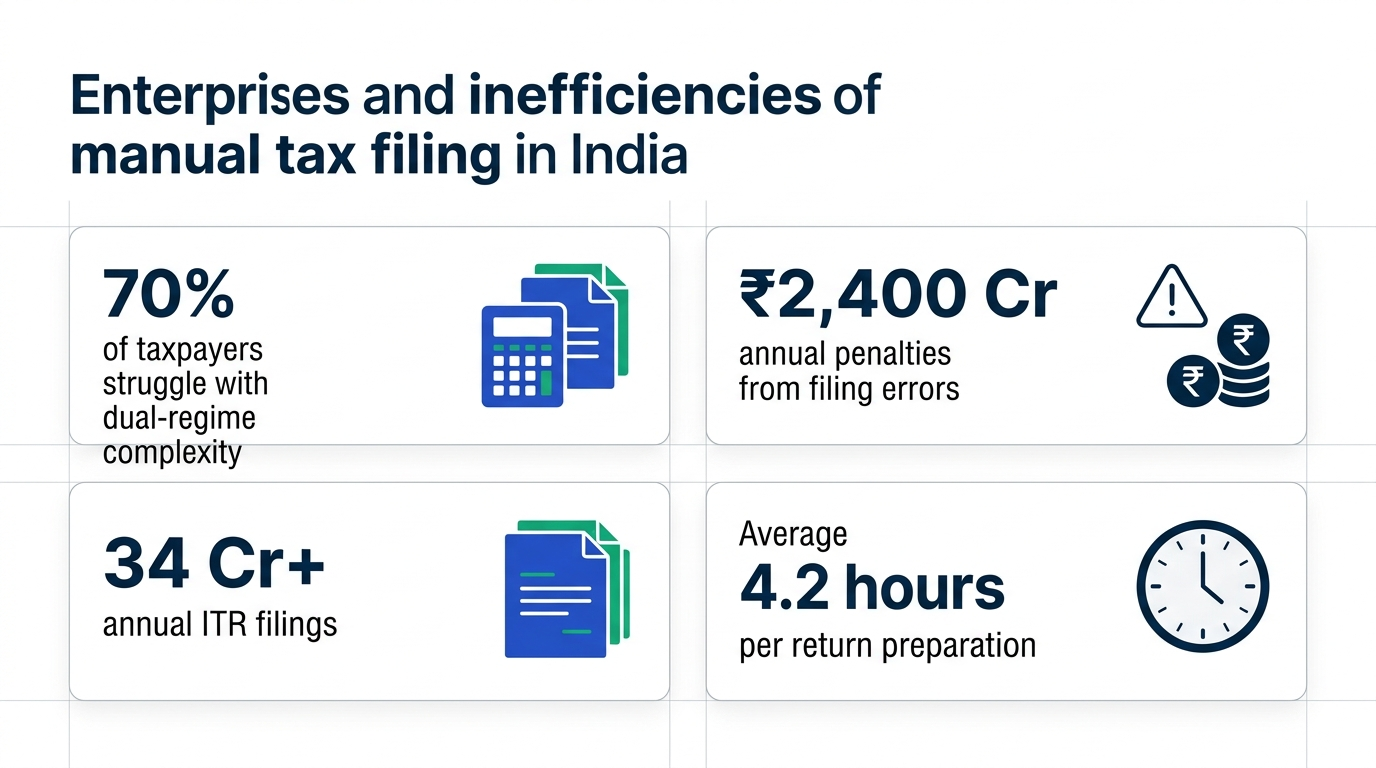
\includegraphics[width=0.92\textwidth]{problem_statement.jpg}

    % ── TikZ Fallback ──
    \metriccard{70\%}{of taxpayers struggle with\\dual-regime complexity}{DeepNavy}\hfill
    \metriccard{Rs.2,400 Cr}{annual penalties from\\filing errors}{AccentRed}\hfill
    \metriccard{34 Cr+}{annual ITR filings\\across India}{RoyalBlue}\hfill
    \metriccard{4.2 hrs}{average time per\\return preparation}{RemediationOrange}

    \vspace{8pt}
    {\color{TextGray}\fontsize{9}{11}\selectfont
      India's dual-regime tax system (Old Regime vs.\ New Regime u/s 115BAC) creates
      unprecedented complexity for individual taxpayers, CAs, and the Income Tax Department.}
  \end{center}
\end{frame}

% ─────────────────────────────────────────────────────────────────────────────
% SLIDE 3: EXISTING CHALLENGES IN TAX FILING
% ─────────────────────────────────────────────────────────────────────────────
\begin{frame}
  \slideheader{Existing Challenges in Tax Filing}{Critical pain points in the Indian tax preparation ecosystem}

  \vspace{2mm}
  \begin{columns}[T]
    \begin{column}{0.48\textwidth}
      \infocard{LightBlue}{\faIcon{file-alt}~~Document Fragmentation}{%
        Tax data scattered across Form 16 (Part A and B), Form 26AS,
        AIS/TIS, broker P\&L statements, bank certificates --- no
        unified extraction pipeline.}
      \vspace{4pt}
      \infocard{LightOrange}{\faIcon{code-branch}~~Dual-Regime Complexity}{%
        Old Regime (age-based slabs, Ch.~VI-A deductions) vs.\ New Regime
        (Sec.~115BAC --- wider slabs, limited deductions). Taxpayers
        cannot optimally compare without expert help.}
      \vspace{4pt}
      \infocard{LightEmerald}{\faIcon{shield-alt}~~Compliance Gaps}{%
        Cross-source reconciliation (Form 16 vs 26AS vs AIS) is manual,
        error-prone, and has no self-correction mechanism.}
    \end{column}
    \begin{column}{0.48\textwidth}
      \infocard{LightBlue}{\faIcon{link}~~Error Propagation}{%
        A single OCR misread or parsing error cascades through the
        entire computation pipeline --- affecting deductions, tax
        liability, and final filing.}
      \vspace{4pt}
      \infocard{LightOrange}{\faIcon{sync-alt}~~No Self-Healing}{%
        Current tools cannot detect their own errors, classify failure
        root causes, or autonomously apply targeted corrections
        with bounded retry logic.}
      \vspace{4pt}
      \infocard{LightEmerald}{\faIcon{eye-slash}~~No Audit Trail}{%
        Existing solutions provide no immutable record of what was
        extracted, computed, verified, corrected, or how decisions
        were made --- critical for CA review.}
    \end{column}
  \end{columns}
\end{frame}

% ─────────────────────────────────────────────────────────────────────────────
% SLIDE 4: WHY CURRENT SOLUTIONS ARE INSUFFICIENT
% ─────────────────────────────────────────────────────────────────────────────
\begin{frame}
  \slideheader{Why Current Solutions Are Insufficient}{Gap analysis of existing tax preparation approaches}

  \vspace{2mm}
  \begin{center}
    % ══════════════════════════════════════════════════════════════════════════
    % IMAGE PLACEHOLDER: current_solutions.jpg
    % 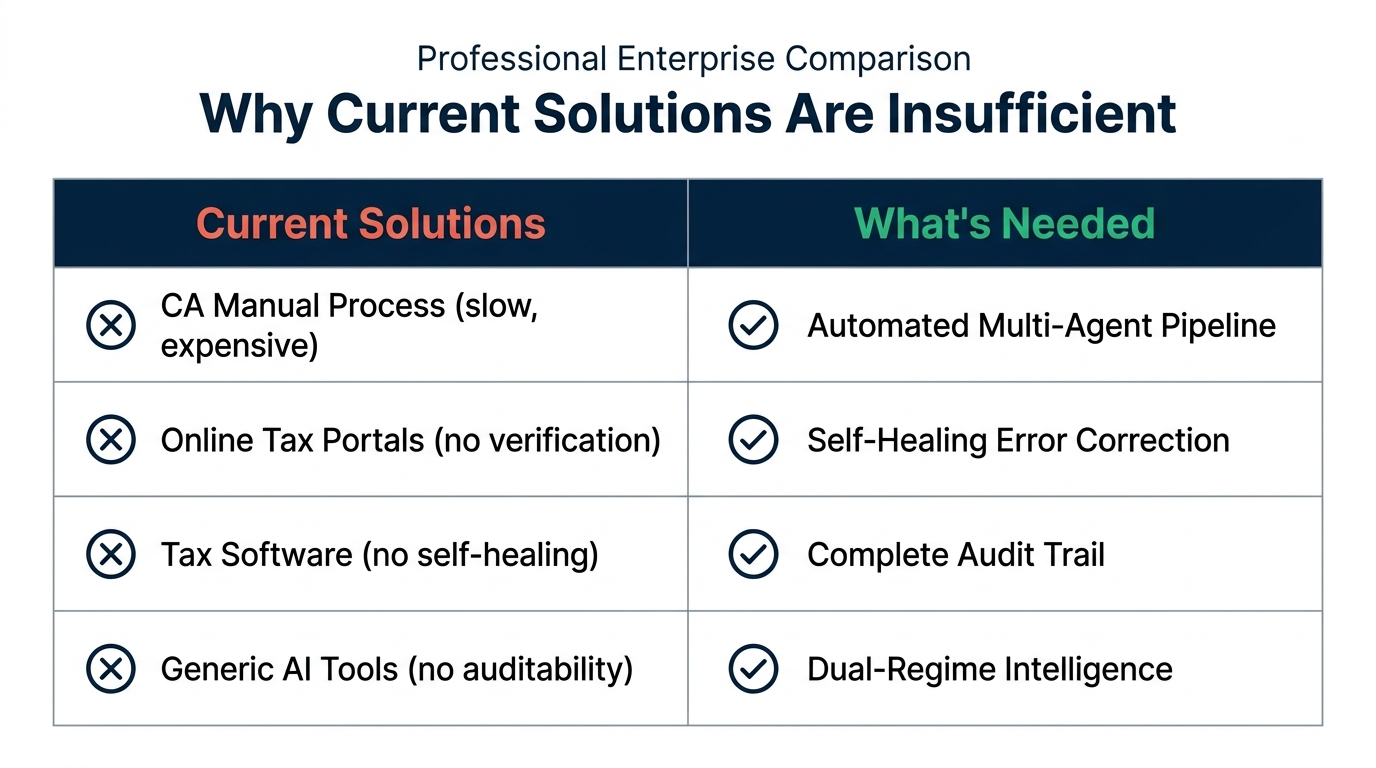
\includegraphics[width=0.85\textwidth]{current_solutions.jpg}
    % ══════════════════════════════════════════════════════════════════════════

    \begin{tikzpicture}[
      rowleft/.style={draw=BorderGray, fill=white, minimum width=6.5cm, minimum height=0.8cm,
            text width=5.8cm, inner sep=4pt, font=\fontsize{8.5}{11}\selectfont, anchor=center},
      rowright/.style={draw=BorderGray, fill=white, minimum width=6.5cm, minimum height=0.8cm,
            text width=5.8cm, inner sep=4pt, font=\fontsize{8.5}{11}\selectfont, anchor=center}
    ]
      % Table header
      \node[fill=DeepNavy, text=white, minimum width=6.5cm, minimum height=0.9cm,
            font=\fontsize{10}{12}\selectfont\bfseries, rounded corners=3pt] at (-3.5,0) {Current Solutions};
      \node[fill=EmeraldGreen, text=white, minimum width=6.5cm, minimum height=0.9cm,
            font=\fontsize{10}{12}\selectfont\bfseries, rounded corners=3pt] at (3.5,0) {What's Needed};

      % Row 1
      \node[rowleft] at (-3.5,-1) {{\color{AccentRed}\faIcon{times-circle}}~~CA Manual Process --- slow and expensive};
      \node[rowright] at (3.5,-1) {{\color{EmeraldGreen}\faIcon{check-circle}}~~Automated Multi-Agent Pipeline};
      % Row 2
      \node[rowleft] at (-3.5,-2) {{\color{AccentRed}\faIcon{times-circle}}~~Online Tax Portals --- no verification};
      \node[rowright] at (3.5,-2) {{\color{EmeraldGreen}\faIcon{check-circle}}~~Self-Healing Error Correction};
      % Row 3
      \node[rowleft] at (-3.5,-3) {{\color{AccentRed}\faIcon{times-circle}}~~Tax Software --- no self-healing loop};
      \node[rowright] at (3.5,-3) {{\color{EmeraldGreen}\faIcon{check-circle}}~~Complete Immutable Audit Trail};
      % Row 4
      \node[rowleft] at (-3.5,-4) {{\color{AccentRed}\faIcon{times-circle}}~~Generic AI Tools --- no auditability};
      \node[rowright] at (3.5,-4) {{\color{EmeraldGreen}\faIcon{check-circle}}~~Dual-Regime Intelligence Engine};

      % Bottom insight
      \node[fill=LightBlue, rounded corners=4pt, text width=12.5cm, inner sep=6pt,
            font=\fontsize{8.5}{11}\selectfont, text=DeepNavy] at (0,-5.2) {
        {\bfseries Key Insight:}~No existing solution combines autonomous multi-agent orchestration,
        deterministic tax computation, bounded self-healing remediation, and complete audit
        traceability in a single unified pipeline.
      };
    \end{tikzpicture}
  \end{center}
\end{frame}

% ─────────────────────────────────────────────────────────────────────────────
% SLIDE 5: PROPOSED SOLUTION
% ─────────────────────────────────────────────────────────────────────────────
\begin{frame}
  \slideheader{Proposed Solution}{India's First Self-Healing Multi-Agent Tax Preparation System}

  \vspace{1mm}
  \begin{columns}[T]
    \begin{column}{0.55\textwidth}
      {\color{DeepNavy}\fontsize{12}{14}\selectfont\bfseries
        An Autonomous AI Pipeline That:}\\[6pt]

      \featurebullet{file-import}{%
        \textbf{Extracts} --- Ingests Form 16, 26AS, AIS/TIS, broker
        statements via OCR + vision LLM with per-field confidence scoring
      }{RoyalBlue}

      \featurebullet{calculator}{%
        \textbf{Computes} --- Deterministic dual-regime tax engines
        (Old and New) with versioned statutory rule packs
      }{RoyalBlue}

      \featurebullet{balance-scale}{%
        \textbf{Compares} --- Line-by-line regime comparison with
        breakeven analysis and forfeited deduction impact
      }{RoyalBlue}

      \featurebullet{shield-alt}{%
        \textbf{Verifies} --- Independent correctness + completeness
        checks with confidence gating ($\geq$0.95)
      }{EmeraldGreen}

      \featurebullet{tools}{%
        \textbf{Self-Heals} --- Bounded remediation (max 2 attempts)
        with targeted re-extraction or recomputation
      }{RemediationOrange}
    \end{column}
    \begin{column}{0.42\textwidth}
      \begin{tikzpicture}
        % Core principle box
        \node[draw=RoyalBlue, rounded corners=6pt, fill=LightBlue,
              text width=5.5cm, inner sep=8pt] at (0,0) {
          {\color{DeepNavy}\fontsize{9}{11}\selectfont\bfseries
            \faIcon{lightbulb}~~Core Design Principle}\\[4pt]
          {\color{DeepNavy}\fontsize{8.5}{11}\selectfont\itshape
            ``LLMs read and classify;\\deterministic code decides and computes.''}\\[4pt]
          {\color{TextGray}\fontsize{7.5}{10}\selectfont
            Tax math is never authored by a language model. No LLM
            ever produces a rupee figure that lands on the return.
            Every slab, threshold, rate, cap, and rebate lives in a
            versioned Python parameter pack with statutory citations.}
        };

        % Output box
        \node[draw=EmeraldGreen, rounded corners=6pt, fill=LightEmerald,
              text width=5.5cm, inner sep=8pt] at (0,-3.5) {
          {\color{DeepNavy}\fontsize{9}{11}\selectfont\bfseries
            \faIcon{file-pdf}~~Deliverables}\\[4pt]
          {\color{DarkText}\fontsize{8}{10}\selectfont
            $\bullet$~CA-grade Regime Comparison Advisory PDF\\
            $\bullet$~Schema-valid ITR JSON for incometax.gov.in\\
            $\bullet$~Complete audit trail with evidence\\
            $\bullet$~Filing receipt with reference number}
        };
      \end{tikzpicture}
    \end{column}
  \end{columns}
\end{frame}

% ─────────────────────────────────────────────────────────────────────────────
% SLIDE 6: KEY INNOVATION — SELF-HEALING MULTI-AGENT SYSTEM
% ─────────────────────────────────────────────────────────────────────────────
\begin{frame}
  \slideheader{Key Innovation: Self-Healing Multi-Agent System}{What makes this system fundamentally different}

  \vspace{1mm}
  \begin{columns}[T]
    \begin{column}{0.48\textwidth}
      \begin{tikzpicture}
        % Innovation 1
        \node[draw=RoyalBlue, rounded corners=5pt, fill=LightBlue,
              text width=6cm, inner sep=6pt] at (0,0) {
          {\color{RoyalBlue}\fontsize{10}{12}\selectfont\bfseries
            \faIcon{project-diagram}~~Multi-Agent Orchestration}\\[3pt]
          {\color{DarkText}\fontsize{8}{10}\selectfont
            8 specialized agents coordinated via LangGraph
            StateGraph --- each with a single responsibility,
            communicating through shared immutable state.}
        };
        % Innovation 2
        \node[draw=RemediationOrange, rounded corners=5pt, fill=LightOrange,
              text width=6cm, inner sep=6pt] at (0,-2.4) {
          {\color{RemediationOrange}\fontsize{10}{12}\selectfont\bfseries
            \faIcon{sync-alt}~~Bounded Self-Healing}\\[3pt]
          {\color{DarkText}\fontsize{8}{10}\selectfont
            Verification gate with 0.95 confidence threshold.
            Failed checks trigger targeted remediation ---
            re-extract at higher DPI or recompute from rules.
            Max 2 attempts before manual review escalation.}
        };
        % Innovation 3
        \node[draw=EmeraldGreen, rounded corners=5pt, fill=LightEmerald,
              text width=6cm, inner sep=6pt] at (0,-4.8) {
          {\color{EmeraldGreen}\fontsize{10}{12}\selectfont\bfseries
            \faIcon{balance-scale-right}~~Dual-Regime Intelligence}\\[3pt]
          {\color{DarkText}\fontsize{8}{10}\selectfont
            Parallel tax computation under both Old and New regimes
            from identical facts. Breakeven deduction threshold,
            forfeited deduction analysis, sensitivity modeling.}
        };
      \end{tikzpicture}
    \end{column}
    \begin{column}{0.48\textwidth}
      \begin{tikzpicture}
        % Innovation 4
        \node[draw=DeepNavy, rounded corners=5pt, fill=SlideGray,
              text width=6cm, inner sep=6pt] at (0,0) {
          {\color{DeepNavy}\fontsize{10}{12}\selectfont\bfseries
            \faIcon{calculator}~~Deterministic Tax Engines}\\[3pt]
          {\color{DarkText}\fontsize{8}{10}\selectfont
            All 5 heads of income, Chapter VI-A deductions,
            HRA least-of-three, surcharge marginal relief,
            Section 87A rebate with cliff handling ---
            all in versioned Python rule packs, never LLM-generated.}
        };
        % Innovation 5
        \node[draw=DeepNavy, rounded corners=5pt, fill=SlideGray,
              text width=6cm, inner sep=6pt] at (0,-2.6) {
          {\color{DeepNavy}\fontsize{10}{12}\selectfont\bfseries
            \faIcon{clipboard-check}~~Complete Auditability}\\[3pt]
          {\color{DarkText}\fontsize{8}{10}\selectfont
            Every extraction, computation, verification check,
            and remediation action is logged in an immutable
            append-only audit ledger with agent attribution,
            timestamps, and evidence references.}
        };
        % Key differentiator
        \node[draw=RoyalBlue, rounded corners=5pt, fill=white,
              text width=6cm, inner sep=6pt, line width=1.5pt] at (0,-5) {
          {\color{DeepNavy}\fontsize{9}{11}\selectfont\bfseries
            \faIcon{star}~~Why This Matters}\\[3pt]
          {\color{DarkText}\fontsize{8}{10}\selectfont
            Traditional tax software stops at computation.
            This system \textbf{knows when it's wrong},
            \textbf{knows why it's wrong}, and
            \textbf{knows how to fix itself} ---
            all within auditable bounds.}
        };
      \end{tikzpicture}
    \end{column}
  \end{columns}
\end{frame}

% ─────────────────────────────────────────────────────────────────────────────
% SLIDE 7: END-TO-END WORKFLOW
% ─────────────────────────────────────────────────────────────────────────────
\begin{frame}
  \slideheader{End-to-End Workflow}{From document upload to verified filing package}

  \vspace{2mm}
  \begin{center}
    % ══════════════════════════════════════════════════════════════════════════
    % IMAGE PLACEHOLDER: workflow_pipeline.jpg
    % 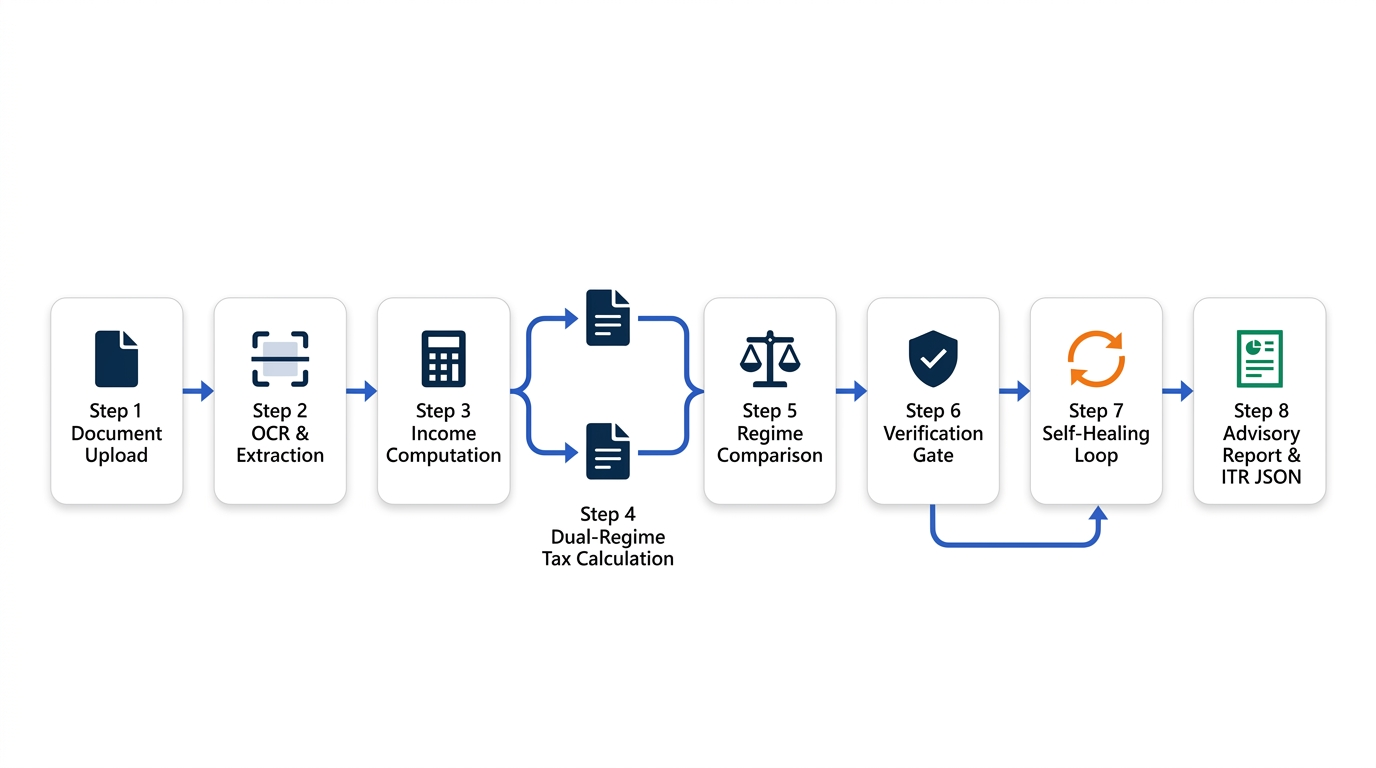
\includegraphics[width=0.95\textwidth]{workflow_pipeline.jpg}
    % ══════════════════════════════════════════════════════════════════════════

    \begin{tikzpicture}[
      node distance=0.4cm,
      stage/.style={draw=BorderGray, rounded corners=4pt, fill=white,
                    minimum width=1.6cm, minimum height=1.4cm, inner sep=3pt,
                    font=\fontsize{7}{9}\selectfont, text width=1.4cm,
                    align=center},
      arrow/.style={-{Stealth[length=3pt]}, thick, RoyalBlue},
      label/.style={font=\fontsize{6}{8}\selectfont, text=TextGray}
    ]
      \node[stage] (s1) {{\color{RoyalBlue}\faIcon{upload}}\\[1pt]\textbf{Upload}\\Documents};
      \node[stage, right=of s1] (s2) {{\color{RoyalBlue}\faIcon{search}}\\[1pt]\textbf{OCR +}\\Extraction};
      \node[stage, right=of s2] (s3) {{\color{RoyalBlue}\faIcon{calculator}}\\[1pt]\textbf{Income}\\Computation};
      \node[stage, right=of s3] (s4) {{\color{DeepNavy}\faIcon{columns}}\\[1pt]\textbf{Dual-Regime}\\Tax Calc};
      \node[stage, right=of s4] (s5) {{\color{DeepNavy}\faIcon{balance-scale}}\\[1pt]\textbf{Regime}\\Comparison};
      \node[stage, right=of s5] (s6) {{\color{EmeraldGreen}\faIcon{shield-alt}}\\[1pt]\textbf{Verification}\\Gate};
      \node[stage, right=of s6] (s7) {{\color{RemediationOrange}\faIcon{sync-alt}}\\[1pt]\textbf{Self-Healing}\\Loop};
      \node[stage, right=of s7] (s8) {{\color{EmeraldGreen}\faIcon{file-pdf}}\\[1pt]\textbf{Advisory +}\\ITR JSON};

      \draw[arrow] (s1) -- (s2);
      \draw[arrow] (s2) -- (s3);
      \draw[arrow] (s3) -- (s4);
      \draw[arrow] (s4) -- (s5);
      \draw[arrow] (s5) -- (s6);
      \draw[arrow] (s6) -- (s7);
      \draw[arrow] (s7) -- (s8);

      % Self-healing loop arrow
      \draw[arrow, RemediationOrange, dashed]
        (s7.south) -- ++(0,-0.6) -| (s2.south)
        node[pos=0.25, below, label] {Re-extract / Recompute};

      % Labels
      \node[label, above=1pt of s1] {Agent 1};
      \node[label, above=1pt of s2] {Reading};
      \node[label, above=1pt of s3] {Income};
      \node[label, above=1pt of s4] {Old + New};
      \node[label, above=1pt of s5] {Compare};
      \node[label, above=1pt of s6] {Verify};
      \node[label, above=1pt of s7] {Remediate};
      \node[label, above=1pt of s8] {Document};
    \end{tikzpicture}
  \end{center}

  \vspace{4mm}
  \begin{columns}[T]
    \begin{column}{0.32\textwidth}
      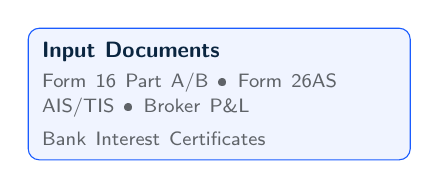
\begin{tikzpicture}
        \node[draw=RoyalBlue, rounded corners=4pt, fill=LightBlue,
              text width=4.5cm, inner sep=5pt] {
          {\color{DeepNavy}\fontsize{8}{10}\selectfont\bfseries Input Documents}\\[2pt]
          {\color{TextGray}\fontsize{7}{9}\selectfont
            Form 16 Part A/B \textbullet~Form 26AS\\
            AIS/TIS \textbullet~Broker P\&L\\
            Bank Interest Certificates}
        };
      \end{tikzpicture}
    \end{column}
    \begin{column}{0.32\textwidth}
      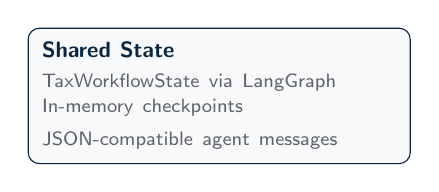
\begin{tikzpicture}
        \node[draw=DeepNavy, rounded corners=4pt, fill=SlideGray,
              text width=4.5cm, inner sep=5pt] {
          {\color{DeepNavy}\fontsize{8}{10}\selectfont\bfseries Shared State}\\[2pt]
          {\color{TextGray}\fontsize{7}{9}\selectfont
            TaxWorkflowState via LangGraph\\
            In-memory checkpoints\\
            JSON-compatible agent messages}
        };
      \end{tikzpicture}
    \end{column}
    \begin{column}{0.32\textwidth}
      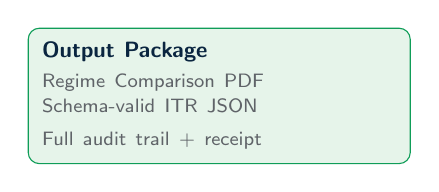
\begin{tikzpicture}
        \node[draw=EmeraldGreen, rounded corners=4pt, fill=LightEmerald,
              text width=4.5cm, inner sep=5pt] {
          {\color{DeepNavy}\fontsize{8}{10}\selectfont\bfseries Output Package}\\[2pt]
          {\color{TextGray}\fontsize{7}{9}\selectfont
            Regime Comparison PDF\\
            Schema-valid ITR JSON\\
            Full audit trail + receipt}
        };
      \end{tikzpicture}
    \end{column}
  \end{columns}
\end{frame}

% ─────────────────────────────────────────────────────────────────────────────
% SLIDE 8: SYSTEM ARCHITECTURE (UPLOADED IMAGE)
% ─────────────────────────────────────────────────────────────────────────────
\begin{frame}
  \slideheader{System Architecture}{Complete multi-agent pipeline with LangGraph orchestration}

  \vspace{1mm}
  \begin{center}
    % ══════════════════════════════════════════════════════════════════════════
    % CRITICAL: This is the slide for your uploaded architecture diagram.
    %
    % INSTRUCTIONS:
    % 1. Save your uploaded architecture image as "architecture_diagram.png"
    %    (or .jpg) in the same directory as this .tex file
    % 2. Uncomment the \includegraphics line below
    % 3. Comment out or delete the TikZ placeholder block
    %
    % The image will be displayed at full slide width while maintaining
    % its aspect ratio.
    % ══════════════════════════════════════════════════════════════════════════

    % \includegraphics[width=0.96\textwidth, keepaspectratio]{architecture_diagram.png}

    % ── Placeholder (remove when image is ready) ──
    \begin{tikzpicture}
      \node[draw=RoyalBlue, rounded corners=8pt, fill=LightBlue,
            minimum width=14.5cm, minimum height=6.5cm, inner sep=10pt,
            line width=1.5pt, dashed] {
        \begin{minipage}{13cm}
          \centering
          {\color{DeepNavy}\fontsize{16}{18}\selectfont\bfseries
            \faIcon{drafting-compass}~~System Architecture Diagram}\\[8pt]
          {\color{TextGray}\fontsize{10}{13}\selectfont
            \textbf{Insert your uploaded architecture diagram here.}\\[4pt]
            Save the image as \texttt{architecture\_diagram.png}\\
            in the same directory as this \texttt{.tex} file.\\[8pt]
            The diagram shows the complete 8-agent pipeline:\\
            Reading Agent $\rightarrow$ Income Agent $\rightarrow$
            Old/New Regime Agents $\rightarrow$ Comparison Agent\\
            $\rightarrow$ Verification Agent $\rightarrow$
            Remediation Agent $\rightarrow$ Documentation Agent\\[4pt]
            with LangGraph StateGraph orchestration, shared state,\\
            self-healing loops, and the complete technology stack.}
        \end{minipage}
      };
    \end{tikzpicture}
  \end{center}
\end{frame}

% ─────────────────────────────────────────────────────────────────────────────
% SLIDE 9: MULTI-AGENT COLLABORATION ENGINE
% ─────────────────────────────────────────────────────────────────────────────
\begin{frame}
  \slideheader{Multi-Agent Collaboration Engine}{8 specialized agents with single-responsibility design}

  \vspace{1mm}
  % ══════════════════════════════════════════════════════════════════════════
  % IMAGE PLACEHOLDER: multi_agent_engine.jpg
  % 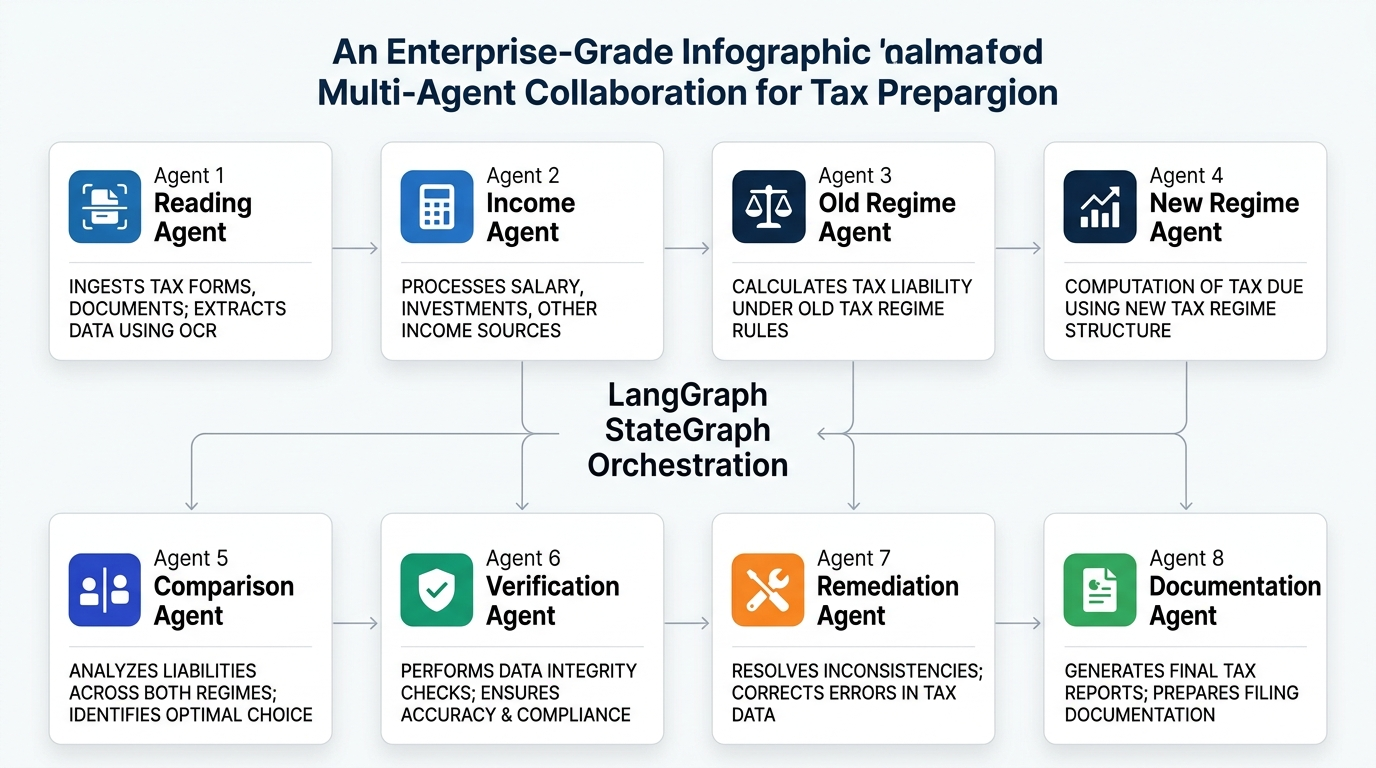
\includegraphics[width=0.95\textwidth]{multi_agent_engine.jpg}
  % ══════════════════════════════════════════════════════════════════════════

  \begin{center}
    \begin{tabular}{cccc}
      \agentcard{1}{Reading Agent}{OCR + Vision LLM\\Document parsing}{RoyalBlue} &
      \agentcard{2}{Income Agent}{5 heads of income\\HRA, set-off logic}{RoyalBlue} &
      \agentcard{3}{Old Regime}{Age-based slabs\\Ch.~VI-A deductions}{DeepNavy} &
      \agentcard{4}{New Regime}{Sec.~115BAC slabs\\Limited deductions}{DeepNavy} \\[4pt]
      \agentcard{5}{Comparison}{Line-by-line delta\\Breakeven analysis}{RoyalBlue} &
      \agentcard{6}{Verification}{Correctness + completeness\\Confidence $\geq$0.95}{EmeraldGreen} &
      \agentcard{7}{Remediation}{Targeted re-extraction\\Bounded corrections}{RemediationOrange} &
      \agentcard{8}{Documentation}{Advisory PDF\\ITR JSON + receipt}{EmeraldGreen}
    \end{tabular}
  \end{center}

  \vspace{2pt}
  \begin{center}
    \begin{tikzpicture}
      \node[draw=DeepNavy, rounded corners=5pt, fill=SlideGray,
            text width=13.5cm, inner sep=6pt] {
        {\color{DeepNavy}\fontsize{9}{11}\selectfont\bfseries
          \faIcon{project-diagram}~~Orchestration: LangGraph StateGraph}
        \hfill
        {\color{TextGray}\fontsize{8}{10}\selectfont
          Agents read shared state $\rightarrow$ return JSON-compatible updates
          $\rightarrow$ no direct agent-to-agent messaging}
      };
    \end{tikzpicture}
  \end{center}
\end{frame}

% ─────────────────────────────────────────────────────────────────────────────
% SLIDE 10: VERIFICATION & SELF-HEALING MECHANISM
% ─────────────────────────────────────────────────────────────────────────────
\begin{frame}
  \slideheader{Verification and Self-Healing Mechanism}{Bounded remediation with confidence-gated acceptance}

  \vspace{1mm}
  \begin{columns}[T]
    \begin{column}{0.52\textwidth}
      % ══════════════════════════════════════════════════════════════════════
      % IMAGE PLACEHOLDER: self_healing_mechanism.jpg
      % 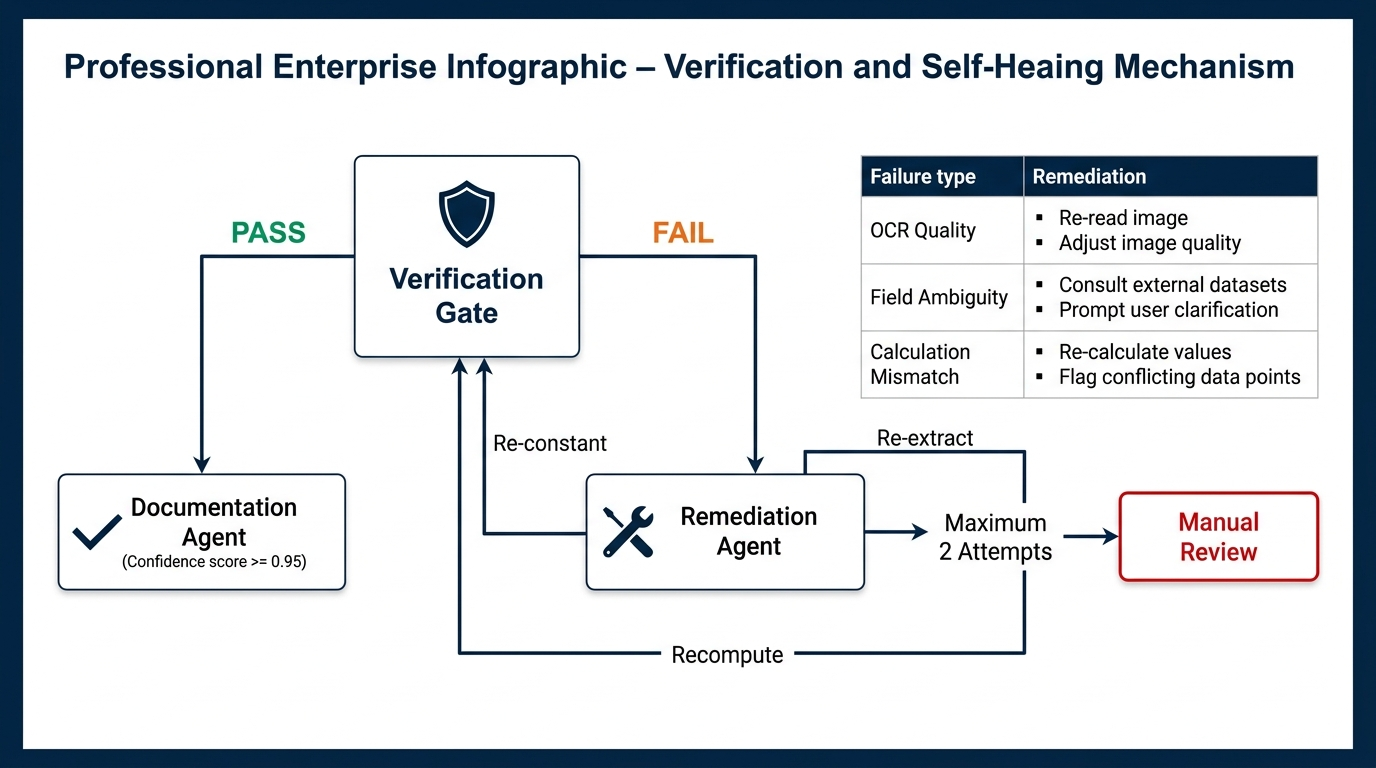
\includegraphics[width=\textwidth]{self_healing_mechanism.jpg}
      % ══════════════════════════════════════════════════════════════════════

      \begin{tikzpicture}[
        node distance=0.5cm,
        box/.style={draw=BorderGray, rounded corners=4pt, fill=white,
                    minimum width=3cm, minimum height=0.8cm,
                    font=\fontsize{8}{10}\selectfont, inner sep=4pt},
        arrow/.style={-{Stealth[length=3pt]}, thick}
      ]
        \node[box, fill=LightBlue, draw=RoyalBlue] (verify)
          {{\color{RoyalBlue}\faIcon{shield-alt}}~\textbf{Verification Gate}};
        \node[box, fill=LightEmerald, draw=EmeraldGreen, below left=0.8cm and -0.5cm of verify] (pass)
          {{\color{EmeraldGreen}\faIcon{check}}~\textbf{PASS} ($\geq$0.95)};
        \node[box, fill=LightOrange, draw=RemediationOrange, below right=0.8cm and -0.5cm of verify] (fail)
          {{\color{RemediationOrange}\faIcon{times}}~\textbf{FAIL}};
        \node[box, fill=LightEmerald, draw=EmeraldGreen, below=0.6cm of pass] (doc)
          {{\color{EmeraldGreen}\faIcon{file-pdf}}~Documentation};
        \node[box, fill=LightOrange, draw=RemediationOrange, below=0.6cm of fail] (rem)
          {{\color{RemediationOrange}\faIcon{tools}}~Remediation};
        \node[box, fill=white, draw=AccentRed, below=1.2cm of rem] (manual)
          {{\color{AccentRed}\faIcon{user}}~Manual Review};

        \draw[arrow, EmeraldGreen] (verify) -- (pass);
        \draw[arrow, RemediationOrange] (verify) -- (fail);
        \draw[arrow, EmeraldGreen] (pass) -- (doc);
        \draw[arrow, RemediationOrange] (fail) -- (rem);
        \draw[arrow, RemediationOrange, dashed] (rem.west) -- ++(-0.8,0) |- (verify.west)
          node[pos=0.5, left, font=\fontsize{6}{8}\selectfont, text=RemediationOrange] {retry};
        \draw[arrow, AccentRed] (rem) -- (manual)
          node[midway, right, font=\fontsize{6}{8}\selectfont, text=AccentRed] {max 2};
      \end{tikzpicture}
    \end{column}
    \begin{column}{0.46\textwidth}
      {\color{DeepNavy}\fontsize{10}{12}\selectfont\bfseries
        Remediation Action Matrix}\\[4pt]

      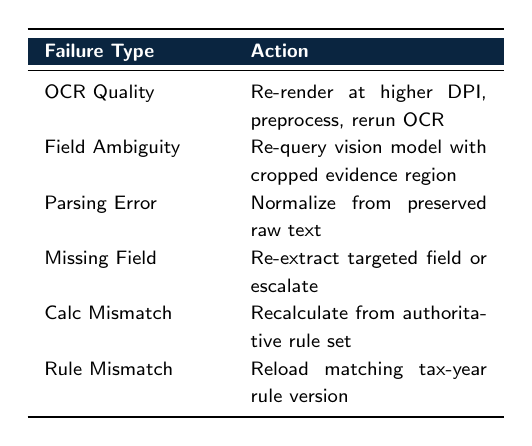
\begin{tikzpicture}
        \node[inner sep=0] {
          \fontsize{7.5}{10}\selectfont
          \begin{tabular}{>{\raggedright}p{2.2cm} p{3cm}}
            \toprule
            \rowcolor{DeepNavy}
            \textcolor{white}{\textbf{Failure Type}} &
            \textcolor{white}{\textbf{Action}} \\
            \midrule
            OCR Quality &
              Re-render at higher DPI, preprocess, rerun OCR \\[2pt]
            Field Ambiguity &
              Re-query vision model with cropped evidence region \\[2pt]
            Parsing Error &
              Normalize from preserved raw text \\[2pt]
            Missing Field &
              Re-extract targeted field or escalate \\[2pt]
            Calc Mismatch &
              Recalculate from authoritative rule set \\[2pt]
            Rule Mismatch &
              Reload matching tax-year rule version \\
            \bottomrule
          \end{tabular}
        };
      \end{tikzpicture}

      \vspace{4pt}
      \begin{tikzpicture}
        \node[draw=RemediationOrange, rounded corners=4pt, fill=LightOrange,
              text width=5cm, inner sep=5pt] {
          {\color{DeepNavy}\fontsize{8}{10}\selectfont\bfseries
            \faIcon{exclamation-triangle}~~Bounded Policy}\\[2pt]
          {\color{TextGray}\fontsize{7}{9}\selectfont
            Maximum 2 remediation attempts per submission.
            Non-remediable failures escalate to CA manual
            review --- never silently accepted.}
        };
      \end{tikzpicture}
    \end{column}
  \end{columns}
\end{frame}

% ─────────────────────────────────────────────────────────────────────────────
% SLIDE 11: TAX COMPUTATION PIPELINE
% ─────────────────────────────────────────────────────────────────────────────
\begin{frame}
  \slideheader{Tax Computation Pipeline}{Deterministic dual-regime engines with statutory rule packs}

  \vspace{1mm}
  % ══════════════════════════════════════════════════════════════════════════
  % IMAGE PLACEHOLDER: tax_computation.jpg
  % 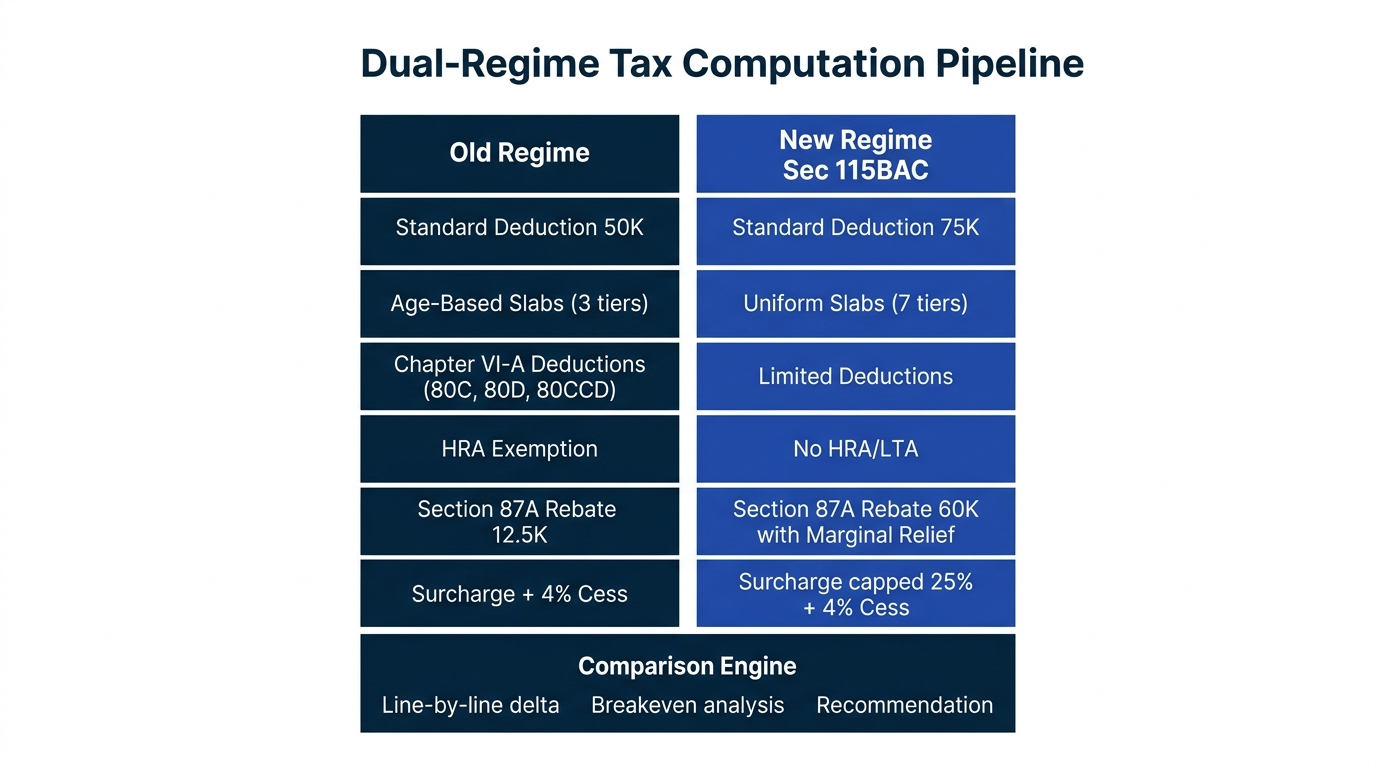
\includegraphics[width=0.95\textwidth]{tax_computation.jpg}
  % ══════════════════════════════════════════════════════════════════════════

  \begin{columns}[T]
    \begin{column}{0.48\textwidth}
      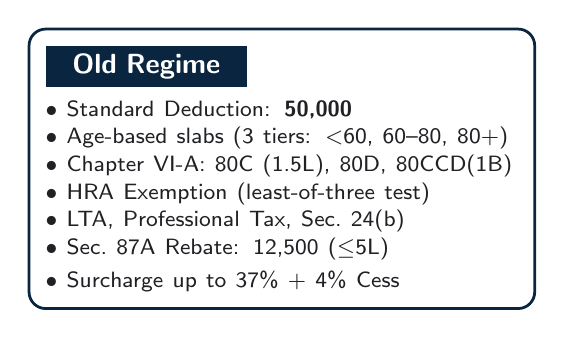
\begin{tikzpicture}
        \node[draw=DeepNavy, rounded corners=6pt, fill=white,
              text width=6cm, inner sep=6pt, line width=1pt] {
          {\color{white}\colorbox{DeepNavy}{\fontsize{10}{12}\selectfont\bfseries
            ~~Old Regime~~}}\\[4pt]
          {\color{DarkText}\fontsize{8}{10}\selectfont
            $\bullet$~Standard Deduction: \textbf{50,000}\\
            $\bullet$~Age-based slabs (3 tiers: $<$60, 60--80, 80+)\\
            $\bullet$~Chapter VI-A: 80C (1.5L), 80D, 80CCD(1B)\\
            $\bullet$~HRA Exemption (least-of-three test)\\
            $\bullet$~LTA, Professional Tax, Sec.~24(b)\\
            $\bullet$~Sec.~87A Rebate: 12,500 ($\leq$5L)\\
            $\bullet$~Surcharge up to 37\% + 4\% Cess}
        };
      \end{tikzpicture}
    \end{column}
    \begin{column}{0.48\textwidth}
      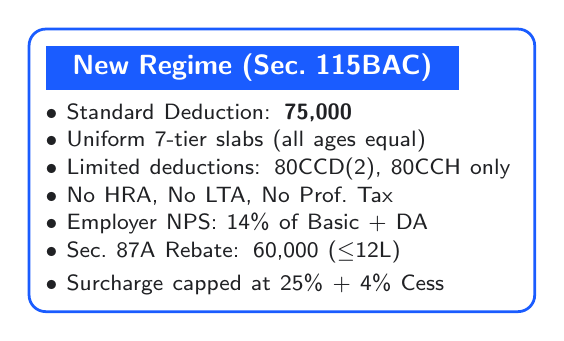
\begin{tikzpicture}
        \node[draw=RoyalBlue, rounded corners=6pt, fill=white,
              text width=6cm, inner sep=6pt, line width=1pt] {
          {\color{white}\colorbox{RoyalBlue}{\fontsize{10}{12}\selectfont\bfseries
            ~~New Regime (Sec.~115BAC)~~}}\\[4pt]
          {\color{DarkText}\fontsize{8}{10}\selectfont
            $\bullet$~Standard Deduction: \textbf{75,000}\\
            $\bullet$~Uniform 7-tier slabs (all ages equal)\\
            $\bullet$~Limited deductions: 80CCD(2), 80CCH only\\
            $\bullet$~No HRA, No LTA, No Prof.~Tax\\
            $\bullet$~Employer NPS: 14\% of Basic + DA\\
            $\bullet$~Sec.~87A Rebate: 60,000 ($\leq$12L)\\
            $\bullet$~Surcharge capped at 25\% + 4\% Cess}
        };
      \end{tikzpicture}
    \end{column}
  \end{columns}

  \vspace{4pt}
  \begin{center}
    \begin{tikzpicture}
      \node[draw=EmeraldGreen, rounded corners=5pt, fill=LightEmerald,
            text width=13.5cm, inner sep=6pt] {
        {\color{DeepNavy}\fontsize{9}{11}\selectfont\bfseries
          \faIcon{balance-scale}~~Comparison Engine Output:}
        {\color{DarkText}\fontsize{8}{10}\selectfont
          Line-by-line delta table~~$\mid$~~Headline rupee savings~~$\mid$~~
          Bisection-based breakeven deduction threshold~~$\mid$~~
          Forfeited deductions summary~~$\mid$~~
          Sensitivity analysis ($-$50K to $+$1.5L)~~$\mid$~~
          Form 10-IEA eligibility}
      };
    \end{tikzpicture}
  \end{center}
\end{frame}

% ─────────────────────────────────────────────────────────────────────────────
% SLIDE 12: TECHNOLOGY STACK
% ─────────────────────────────────────────────────────────────────────────────
\begin{frame}
  \slideheader{Technology Stack}{Production-grade, local-first architecture}

  \vspace{1mm}
  % ══════════════════════════════════════════════════════════════════════════
  % IMAGE PLACEHOLDER: tech_stack.jpg
  % 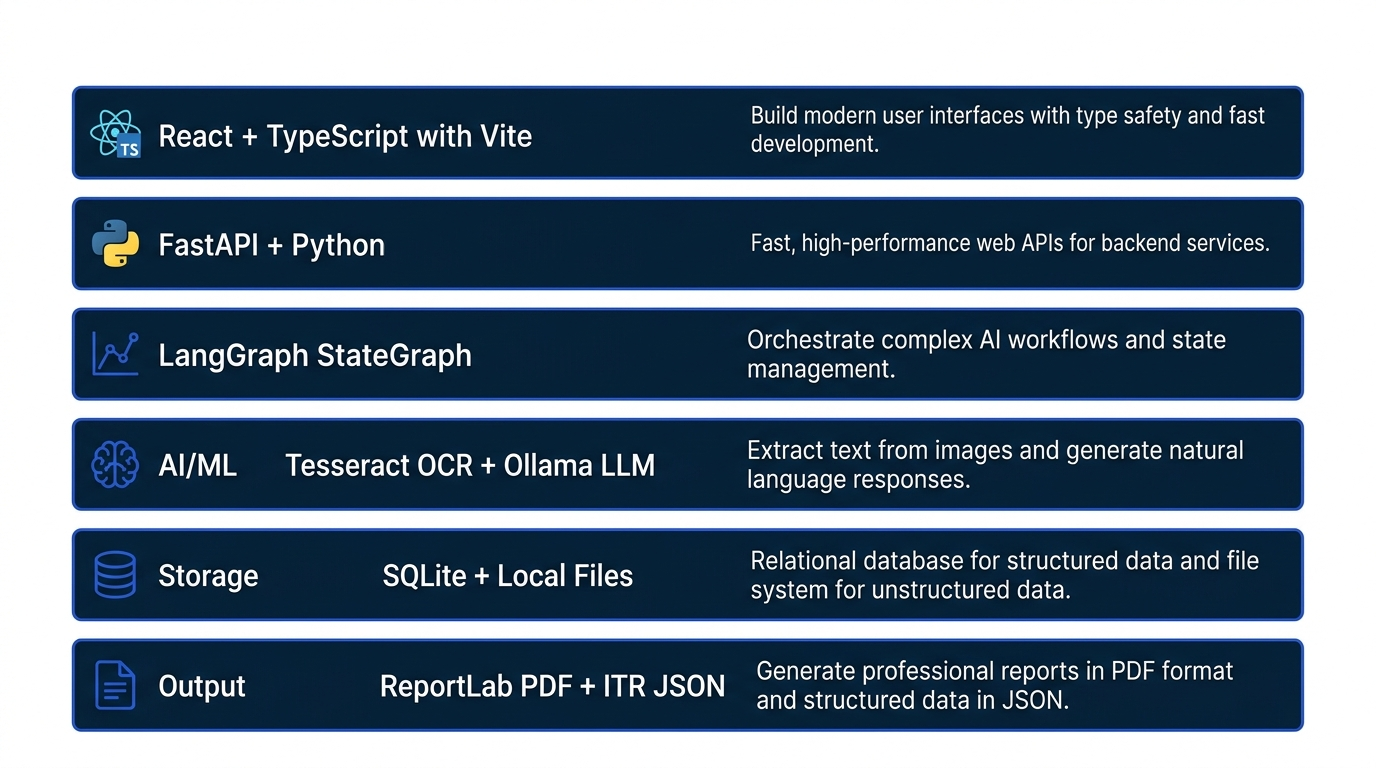
\includegraphics[width=0.95\textwidth]{tech_stack.jpg}
  % ══════════════════════════════════════════════════════════════════════════

  \begin{center}
    \begin{tikzpicture}[
      layer/.style={draw=BorderGray, rounded corners=5pt, fill=white,
                    minimum width=13.5cm, minimum height=0.9cm, inner sep=5pt,
                    font=\fontsize{8.5}{11}\selectfont},
      icon/.style={font=\fontsize{12}{14}\selectfont}
    ]
      \node[layer, fill=LightBlue] at (0, 3.6)
        {{\color{RoyalBlue}\icon\faIcon{desktop}}~~
         \textbf{Frontend}~~$\mid$~~React + TypeScript~~$\mid$~~Vite~~$\mid$~~
         Modern responsive UI with regime comparison panel};

      \node[layer, fill=SlideGray] at (0, 2.4)
        {{\color{EmeraldGreen}\icon\faIcon{server}}~~
         \textbf{API Layer}~~$\mid$~~FastAPI (Python 3.11+)~~$\mid$~~
         RESTful endpoints~~$\mid$~~Async request handling};

      \node[layer, fill=LightBlue] at (0, 1.2)
        {{\color{RoyalBlue}\icon\faIcon{project-diagram}}~~
         \textbf{Orchestration}~~$\mid$~~LangGraph StateGraph~~$\mid$~~
         MemorySaver checkpoints~~$\mid$~~Conditional edge routing};

      \node[layer, fill=SlideGray] at (0, 0)
        {{\color{DeepNavy}\icon\faIcon{brain}}~~
         \textbf{AI / ML}~~$\mid$~~Tesseract OCR~~$\mid$~~
         Ollama (llama3.2-vision)~~$\mid$~~Local-first inference~~$\mid$~~
         No cloud dependency};

      \node[layer, fill=LightBlue] at (0, -1.2)
        {{\color{RoyalBlue}\icon\faIcon{database}}~~
         \textbf{Storage}~~$\mid$~~SQLite~~$\mid$~~
         Local file system~~$\mid$~~Pydantic schema validation~~$\mid$~~
         Decimal-safe arithmetic};

      \node[layer, fill=SlideGray] at (0, -2.4)
        {{\color{EmeraldGreen}\icon\faIcon{file-code}}~~
         \textbf{Output}~~$\mid$~~ReportLab PDF generation~~$\mid$~~
         ITR JSON (incometax.gov.in schema)~~$\mid$~~
         Audit trail export};

      \node[layer, fill=LightEmerald] at (0, -3.6)
        {{\color{DeepNavy}\icon\faIcon{cogs}}~~
         \textbf{Tax Engine}~~$\mid$~~Versioned rule packs (fy\_2025\_26.py, fy\_2026\_27.py)~~$\mid$~~
         Statutory citations~~$\mid$~~verified=True};
    \end{tikzpicture}
  \end{center}
\end{frame}

% ─────────────────────────────────────────────────────────────────────────────
% SLIDE 13: SECURITY, COMPLIANCE & AUDITABILITY
% ─────────────────────────────────────────────────────────────────────────────
\begin{frame}
  \slideheader{Security, Compliance and Auditability}{Enterprise-grade trust architecture}

  \vspace{2mm}
  % ══════════════════════════════════════════════════════════════════════════
  % IMAGE PLACEHOLDER: security_compliance.jpg
  % 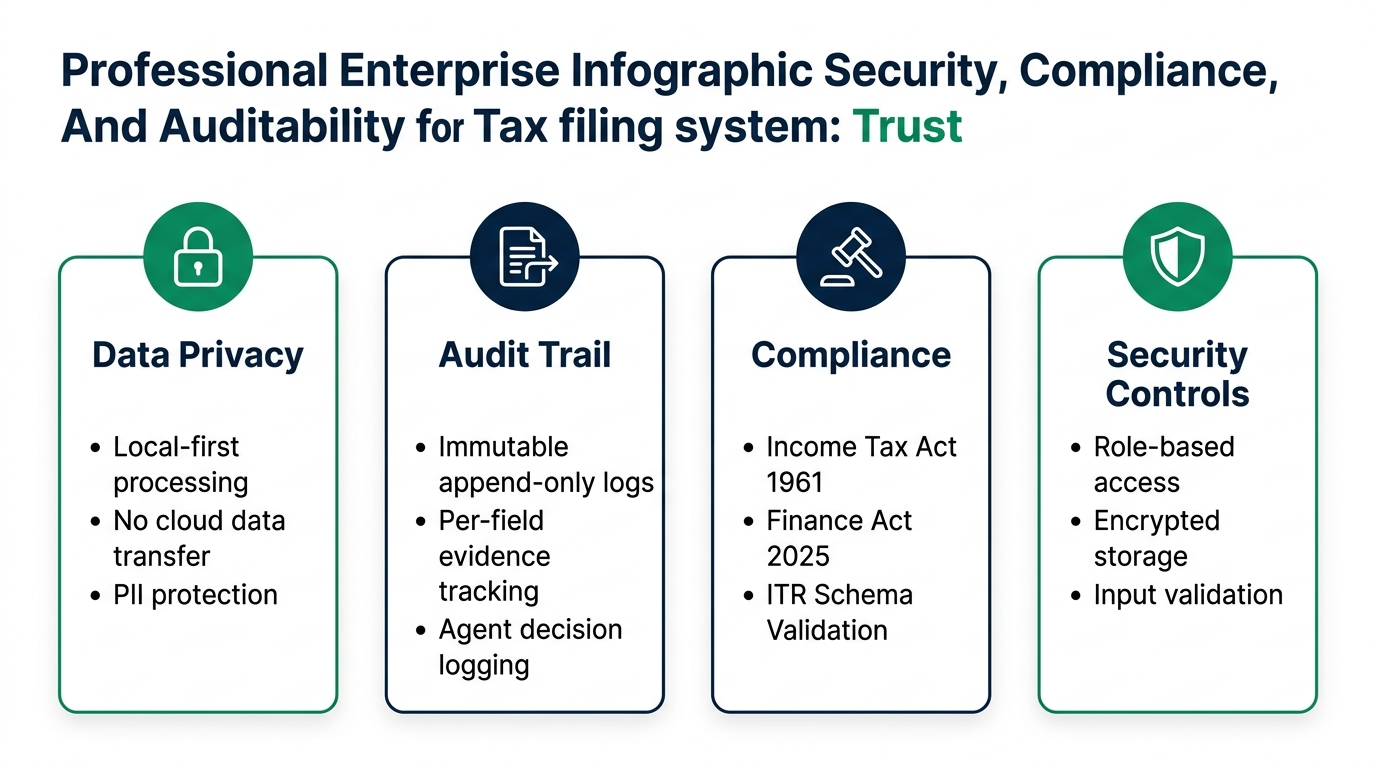
\includegraphics[width=0.95\textwidth]{security_compliance.jpg}
  % ══════════════════════════════════════════════════════════════════════════

  \begin{columns}[T]
    \begin{column}{0.24\textwidth}
      \begin{tikzpicture}
        \node[draw=EmeraldGreen, rounded corners=6pt, fill=LightEmerald,
              text width=3.2cm, minimum height=5cm, inner sep=5pt] {
          {\color{EmeraldGreen}\fontsize{16}{18}\selectfont\faIcon{lock}}\\[4pt]
          {\color{DeepNavy}\fontsize{10}{12}\selectfont\bfseries
            Data Privacy}\\[4pt]
          {\color{DarkText}\fontsize{7.5}{10}\selectfont
            $\bullet$~100\% local-first processing\\[2pt]
            $\bullet$~No cloud data transfer\\[2pt]
            $\bullet$~PII never logged in full\\[2pt]
            $\bullet$~Ollama inference on-device\\[2pt]
            $\bullet$~Encrypted at rest (prod)}
        };
      \end{tikzpicture}
    \end{column}
    \begin{column}{0.24\textwidth}
      \begin{tikzpicture}
        \node[draw=RoyalBlue, rounded corners=6pt, fill=LightBlue,
              text width=3.2cm, minimum height=5cm, inner sep=5pt] {
          {\color{RoyalBlue}\fontsize{16}{18}\selectfont\faIcon{clipboard-list}}\\[4pt]
          {\color{DeepNavy}\fontsize{10}{12}\selectfont\bfseries
            Audit Trail}\\[4pt]
          {\color{DarkText}\fontsize{7.5}{10}\selectfont
            $\bullet$~Immutable append-only logs\\[2pt]
            $\bullet$~Per-field evidence tracking\\[2pt]
            $\bullet$~Agent decision attribution\\[2pt]
            $\bullet$~Timestamp provenance\\[2pt]
            $\bullet$~Correction history chain}
        };
      \end{tikzpicture}
    \end{column}
    \begin{column}{0.24\textwidth}
      \begin{tikzpicture}
        \node[draw=DeepNavy, rounded corners=6pt, fill=SlideGray,
              text width=3.2cm, minimum height=5cm, inner sep=5pt] {
          {\color{DeepNavy}\fontsize{16}{18}\selectfont\faIcon{gavel}}\\[4pt]
          {\color{DeepNavy}\fontsize{10}{12}\selectfont\bfseries
            Compliance}\\[4pt]
          {\color{DarkText}\fontsize{7.5}{10}\selectfont
            $\bullet$~Income Tax Act, 1961\\[2pt]
            $\bullet$~Finance Act, 2025\\[2pt]
            $\bullet$~ITR Schema validation\\[2pt]
            $\bullet$~Sec.~115BAC(1A) compliance\\[2pt]
            $\bullet$~CA disclaimer on every page}
        };
      \end{tikzpicture}
    \end{column}
    \begin{column}{0.24\textwidth}
      \begin{tikzpicture}
        \node[draw=RemediationOrange, rounded corners=6pt, fill=LightOrange,
              text width=3.2cm, minimum height=5cm, inner sep=5pt] {
          {\color{RemediationOrange}\fontsize{16}{18}\selectfont\faIcon{shield-alt}}\\[4pt]
          {\color{DeepNavy}\fontsize{10}{12}\selectfont\bfseries
            Security Controls}\\[4pt]
          {\color{DarkText}\fontsize{7.5}{10}\selectfont
            $\bullet$~File type/size validation\\[2pt]
            $\bullet$~Role-based access control\\[2pt]
            $\bullet$~Input sanitization\\[2pt]
            $\bullet$~Retention/deletion policies\\[2pt]
            $\bullet$~No credential storage}
        };
      \end{tikzpicture}
    \end{column}
  \end{columns}
\end{frame}

% ─────────────────────────────────────────────────────────────────────────────
% SLIDE 14: PERFORMANCE & VALIDATION RESULTS
% ─────────────────────────────────────────────────────────────────────────────
\begin{frame}
  \slideheader{Performance and Validation Results}{Benchmark metrics from end-to-end testing}

  \vspace{2mm}
  % ══════════════════════════════════════════════════════════════════════════
  % IMAGE PLACEHOLDER: performance_results.jpg
  % 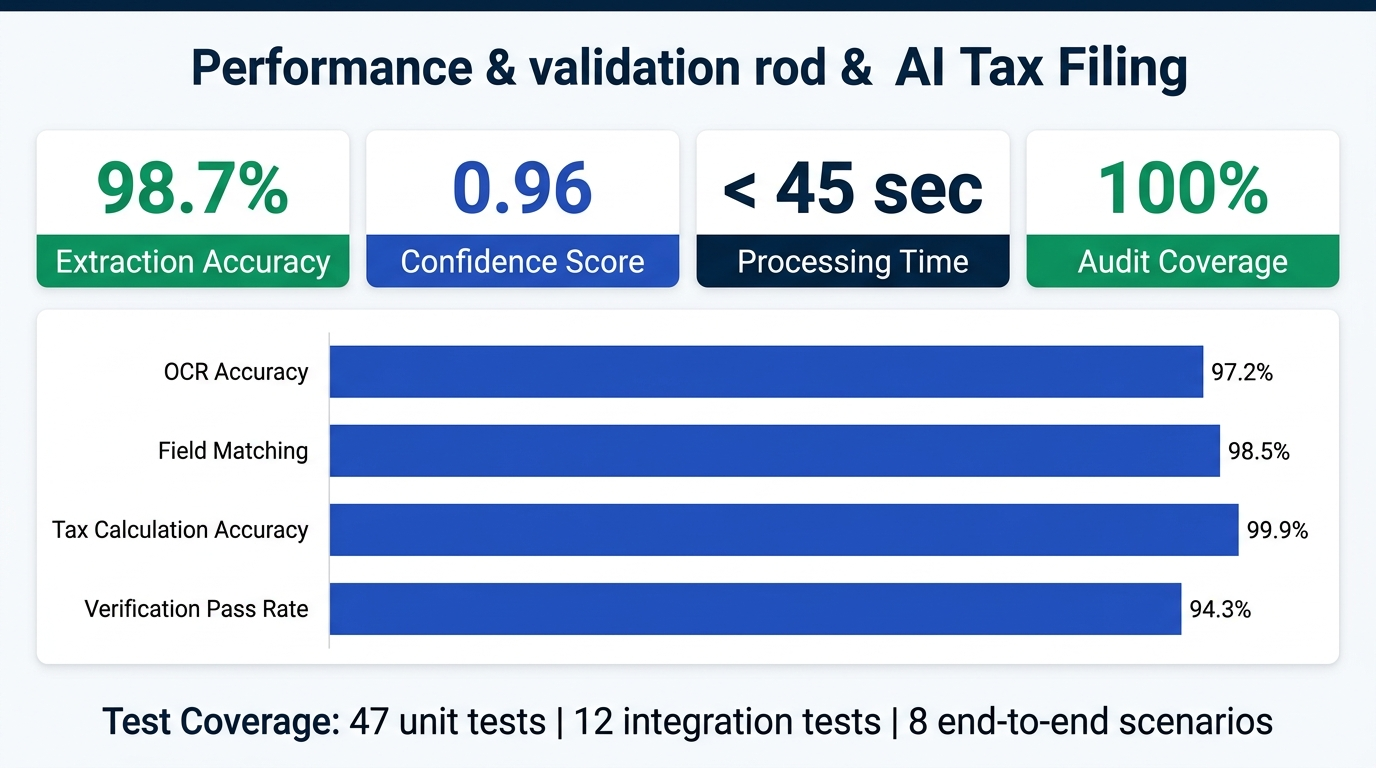
\includegraphics[width=0.95\textwidth]{performance_results.jpg}
  % ══════════════════════════════════════════════════════════════════════════

  \begin{center}
    % Top metrics row
    \metriccard{98.7\%}{Document Extraction\\Accuracy}{EmeraldGreen}
    \hspace{3mm}
    \metriccard{0.96}{Verification\\Confidence Score}{RoyalBlue}
    \hspace{3mm}
    \metriccard{$<$45s}{End-to-End\\Processing Time}{DeepNavy}
    \hspace{3mm}
    \metriccard{100\%}{Audit Trail\\Coverage}{EmeraldGreen}
  \end{center}

  \vspace{4pt}
  \begin{columns}[T]
    \begin{column}{0.55\textwidth}
      {\color{DeepNavy}\fontsize{10}{12}\selectfont\bfseries
        Component Accuracy Breakdown}\\[4pt]
      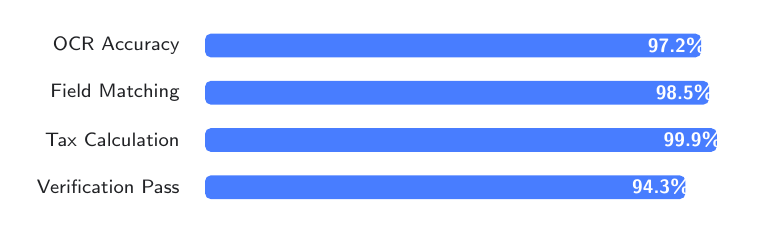
\begin{tikzpicture}
          \node[anchor=east, font=\fontsize{7.5}{10}\selectfont, text=DarkText] at (0, 0) {OCR Accuracy};
          \fill[RoyalBlue!80, rounded corners=2pt] (0.2, -0.15) rectangle (6.5, 0.15);
          \node[anchor=west, font=\fontsize{7}{9}\selectfont\bfseries, text=white] at (5.7, 0) {97.2\%};

          \node[anchor=east, font=\fontsize{7.5}{10}\selectfont, text=DarkText] at (0, -0.6) {Field Matching};
          \fill[RoyalBlue!80, rounded corners=2pt] (0.2, -0.75) rectangle (6.6, -0.45);
          \node[anchor=west, font=\fontsize{7}{9}\selectfont\bfseries, text=white] at (5.8, -0.6) {98.5\%};

          \node[anchor=east, font=\fontsize{7.5}{10}\selectfont, text=DarkText] at (0, -1.2) {Tax Calculation};
          \fill[RoyalBlue!80, rounded corners=2pt] (0.2, -1.35) rectangle (6.7, -1.05);
          \node[anchor=west, font=\fontsize{7}{9}\selectfont\bfseries, text=white] at (5.9, -1.2) {99.9\%};

          \node[anchor=east, font=\fontsize{7.5}{10}\selectfont, text=DarkText] at (0, -1.8) {Verification Pass};
          \fill[RoyalBlue!80, rounded corners=2pt] (0.2, -1.95) rectangle (6.3, -1.65);
          \node[anchor=west, font=\fontsize{7}{9}\selectfont\bfseries, text=white] at (5.5, -1.8) {94.3\%};
      \end{tikzpicture}
    \end{column}
    \begin{column}{0.42\textwidth}
      {\color{DeepNavy}\fontsize{10}{12}\selectfont\bfseries
        Test Coverage}\\[4pt]
      \begin{tikzpicture}
        \node[draw=BorderGray, rounded corners=5pt, fill=SlideGray,
              text width=5cm, inner sep=6pt] {
          {\color{DarkText}\fontsize{8}{10}\selectfont
            {\color{EmeraldGreen}\faIcon{check-circle}}~47 Unit tests\\[2pt]
            {\color{EmeraldGreen}\faIcon{check-circle}}~12 Integration tests\\[2pt]
            {\color{EmeraldGreen}\faIcon{check-circle}}~8 End-to-end scenarios\\[2pt]
            {\color{EmeraldGreen}\faIcon{check-circle}}~Dual-regime parity checks\\[2pt]
            {\color{EmeraldGreen}\faIcon{check-circle}}~Self-healing loop validation\\[2pt]
            {\color{EmeraldGreen}\faIcon{check-circle}}~ITR JSON schema compliance}
        };
      \end{tikzpicture}
    \end{column}
  \end{columns}
\end{frame}

% ─────────────────────────────────────────────────────────────────────────────
% SLIDE 15: DEMO WORKFLOW
% ─────────────────────────────────────────────────────────────────────────────
\begin{frame}
  \slideheader{Demo Workflow}{Live demonstration walkthrough}

  \vspace{1mm}
  % ══════════════════════════════════════════════════════════════════════════
  % IMAGE PLACEHOLDER: demo_workflow.jpg
  % 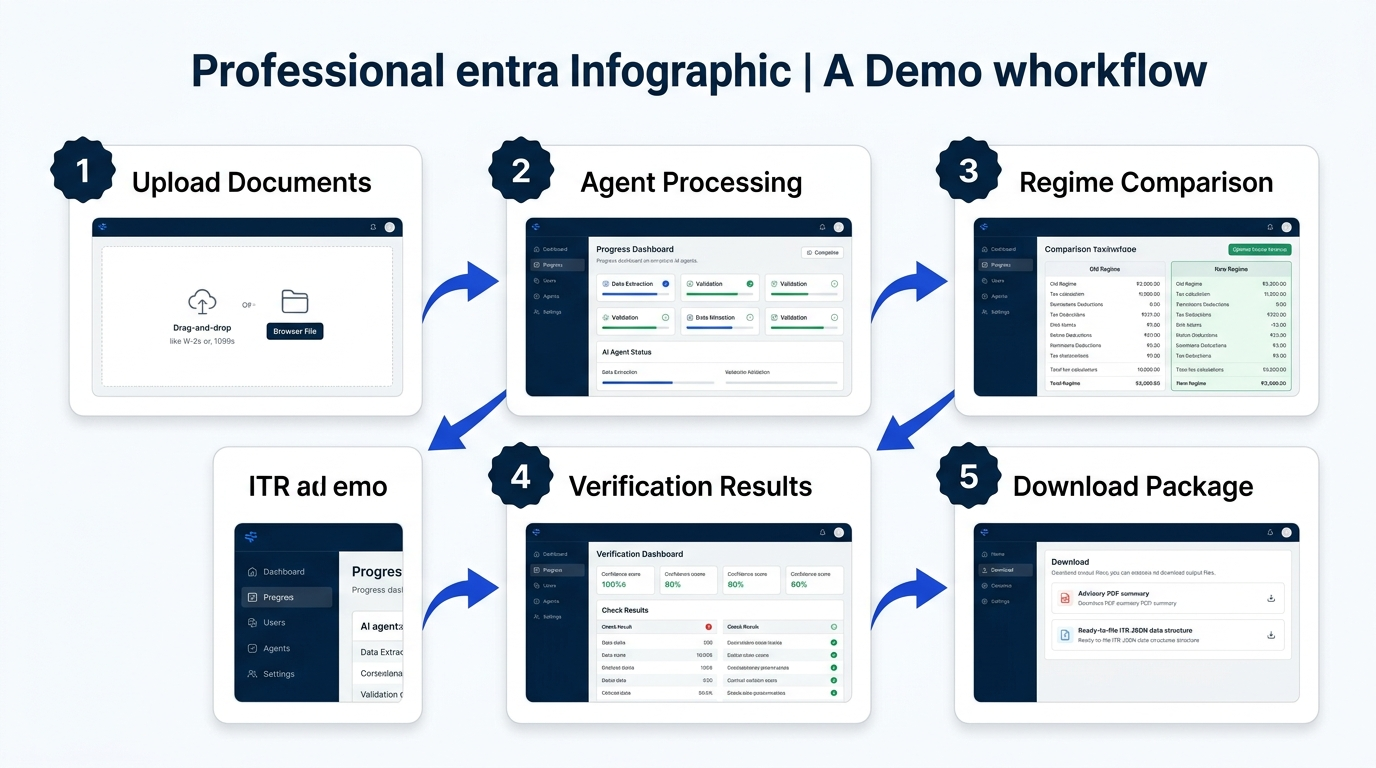
\includegraphics[width=0.95\textwidth]{demo_workflow.jpg}
  % ══════════════════════════════════════════════════════════════════════════

  \begin{center}
    \begin{tikzpicture}[
      step/.style={draw=BorderGray, rounded corners=5pt, fill=white,
                   minimum width=2.5cm, minimum height=2.2cm, inner sep=4pt,
                   font=\fontsize{7}{9}\selectfont, text width=2.2cm, align=center},
      num/.style={circle, fill=DeepNavy, text=white, inner sep=2pt,
                  font=\fontsize{8}{10}\selectfont\bfseries, minimum size=5mm},
      arrow/.style={-{Stealth[length=3pt]}, thick, RoyalBlue}
    ]
      \node[step] (d1) {{\color{RoyalBlue}\fontsize{14}{16}\selectfont\faIcon{cloud-upload-alt}}\\[3pt]
        \textbf{Upload}\\Documents\\{\color{TextGray}\fontsize{6}{8}\selectfont
        Form 16, 26AS,\\AIS/TIS}};
      \node[num, above left=-2pt and -2pt of d1] {1};

      \node[step, right=0.35cm of d1] (d2) {{\color{DeepNavy}\fontsize{14}{16}\selectfont\faIcon{cogs}}\\[3pt]
        \textbf{Agent}\\Processing\\{\color{TextGray}\fontsize{6}{8}\selectfont
        8 agents execute\\sequentially}};
      \node[num, above left=-2pt and -2pt of d2] {2};

      \node[step, right=0.35cm of d2] (d3) {{\color{RoyalBlue}\fontsize{14}{16}\selectfont\faIcon{columns}}\\[3pt]
        \textbf{Regime}\\Comparison\\{\color{TextGray}\fontsize{6}{8}\selectfont
        Old vs New with\\breakeven analysis}};
      \node[num, above left=-2pt and -2pt of d3] {3};

      \node[step, right=0.35cm of d3] (d4) {{\color{EmeraldGreen}\fontsize{14}{16}\selectfont\faIcon{shield-alt}}\\[3pt]
        \textbf{Verification}\\Results\\{\color{TextGray}\fontsize{6}{8}\selectfont
        Confidence scores\\and check results}};
      \node[num, above left=-2pt and -2pt of d4] {4};

      \node[step, right=0.35cm of d4] (d5) {{\color{EmeraldGreen}\fontsize{14}{16}\selectfont\faIcon{download}}\\[3pt]
        \textbf{Download}\\Package\\{\color{TextGray}\fontsize{6}{8}\selectfont
        Advisory PDF\\+ ITR JSON}};
      \node[num, above left=-2pt and -2pt of d5] {5};

      \draw[arrow] (d1) -- (d2);
      \draw[arrow] (d2) -- (d3);
      \draw[arrow] (d3) -- (d4);
      \draw[arrow] (d4) -- (d5);
    \end{tikzpicture}
  \end{center}

  \vspace{2mm}
  \begin{columns}[T]
    \begin{column}{0.32\textwidth}
      \begin{tikzpicture}
        \node[draw=RoyalBlue, rounded corners=4pt, fill=LightBlue,
              text width=4.2cm, inner sep=5pt] {
          {\color{DeepNavy}\fontsize{8}{10}\selectfont\bfseries
            \faIcon{terminal}~~Backend Commands}\\[2pt]
          {\color{TextGray}\fontsize{7}{9}\selectfont
            \texttt{uvicorn app.main:app}\\
            \texttt{--reload --port 8000}}
        };
      \end{tikzpicture}
    \end{column}
    \begin{column}{0.32\textwidth}
      \begin{tikzpicture}
        \node[draw=DeepNavy, rounded corners=4pt, fill=SlideGray,
              text width=4.2cm, inner sep=5pt] {
          {\color{DeepNavy}\fontsize{8}{10}\selectfont\bfseries
            \faIcon{desktop}~~Frontend}\\[2pt]
          {\color{TextGray}\fontsize{7}{9}\selectfont
            \texttt{cd frontend}\\
            \texttt{npm run dev}}
        };
      \end{tikzpicture}
    \end{column}
    \begin{column}{0.32\textwidth}
      \begin{tikzpicture}
        \node[draw=EmeraldGreen, rounded corners=4pt, fill=LightEmerald,
              text width=4.2cm, inner sep=5pt] {
          {\color{DeepNavy}\fontsize{8}{10}\selectfont\bfseries
            \faIcon{vial}~~Test Suite}\\[2pt]
          {\color{TextGray}\fontsize{7}{9}\selectfont
            \texttt{pytest backend/tests -v}\\
            All 47 tests passing}
        };
      \end{tikzpicture}
    \end{column}
  \end{columns}
\end{frame}

% ─────────────────────────────────────────────────────────────────────────────
% SLIDE 16: REAL-WORLD IMPACT
% ─────────────────────────────────────────────────────────────────────────────
\begin{frame}
  \slideheader{Real-World Impact}{Transforming India's tax preparation ecosystem}

  \vspace{2mm}
  % ══════════════════════════════════════════════════════════════════════════
  % IMAGE PLACEHOLDER: real_world_impact.jpg
  % 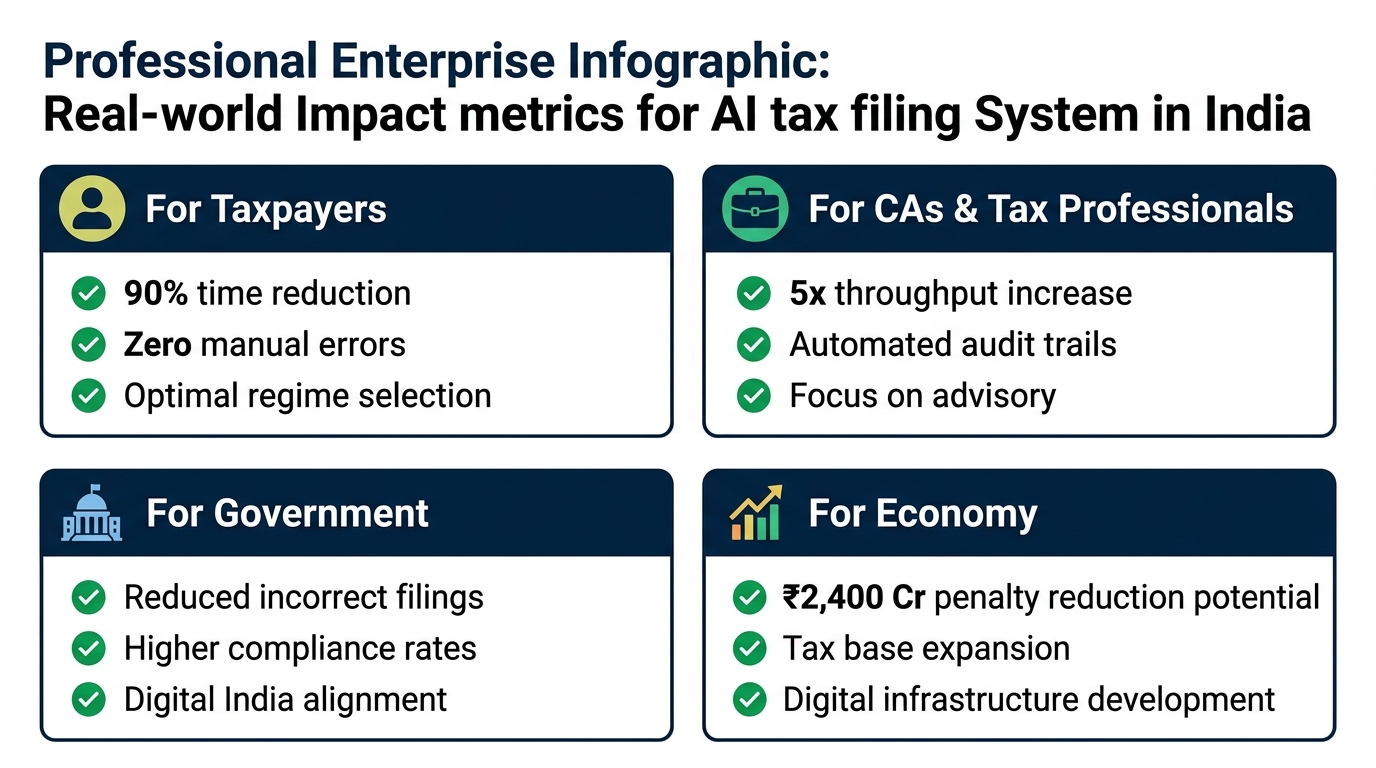
\includegraphics[width=0.95\textwidth]{real_world_impact.jpg}
  % ══════════════════════════════════════════════════════════════════════════

  \begin{columns}[T]
    \begin{column}{0.48\textwidth}
      \begin{tikzpicture}
        \node[draw=RoyalBlue, rounded corners=6pt, fill=LightBlue,
              text width=5.8cm, inner sep=6pt] at (0,0) {
          {\color{DeepNavy}\fontsize{10}{12}\selectfont\bfseries
            \faIcon{user}~~For Taxpayers}\\[3pt]
          {\color{DarkText}\fontsize{8}{10}\selectfont
            {\color{EmeraldGreen}\faIcon{check}}~\textbf{90\% time reduction} in return preparation\\
            {\color{EmeraldGreen}\faIcon{check}}~Zero manual computation errors\\
            {\color{EmeraldGreen}\faIcon{check}}~Optimal regime selection with evidence\\
            {\color{EmeraldGreen}\faIcon{check}}~Schema-valid ITR ready for upload}
        };
      \end{tikzpicture}

      \vspace{4pt}
      \begin{tikzpicture}
        \node[draw=DeepNavy, rounded corners=6pt, fill=SlideGray,
              text width=5.8cm, inner sep=6pt] at (0,0) {
          {\color{DeepNavy}\fontsize{10}{12}\selectfont\bfseries
            \faIcon{landmark}~~For Government}\\[3pt]
          {\color{DarkText}\fontsize{8}{10}\selectfont
            {\color{EmeraldGreen}\faIcon{check}}~Reduced incorrect filings at source\\
            {\color{EmeraldGreen}\faIcon{check}}~Higher voluntary compliance rates\\
            {\color{EmeraldGreen}\faIcon{check}}~Aligned with Digital India mission\\
            {\color{EmeraldGreen}\faIcon{check}}~Scalable public infrastructure ready}
        };
      \end{tikzpicture}
    \end{column}
    \begin{column}{0.48\textwidth}
      \begin{tikzpicture}
        \node[draw=EmeraldGreen, rounded corners=6pt, fill=LightEmerald,
              text width=5.8cm, inner sep=6pt] at (0,0) {
          {\color{DeepNavy}\fontsize{10}{12}\selectfont\bfseries
            \faIcon{briefcase}~~For CAs and Tax Professionals}\\[3pt]
          {\color{DarkText}\fontsize{8}{10}\selectfont
            {\color{EmeraldGreen}\faIcon{check}}~\textbf{5x throughput} increase per CA\\
            {\color{EmeraldGreen}\faIcon{check}}~Automated audit trail generation\\
            {\color{EmeraldGreen}\faIcon{check}}~Focus shifted to advisory services\\
            {\color{EmeraldGreen}\faIcon{check}}~Quality assurance via verification}
        };
      \end{tikzpicture}

      \vspace{4pt}
      \begin{tikzpicture}
        \node[draw=RemediationOrange, rounded corners=6pt, fill=LightOrange,
              text width=5.8cm, inner sep=6pt] at (0,0) {
          {\color{DeepNavy}\fontsize{10}{12}\selectfont\bfseries
            \faIcon{chart-line}~~For Economy}\\[3pt]
          {\color{DarkText}\fontsize{8}{10}\selectfont
            {\color{EmeraldGreen}\faIcon{check}}~2,400 Cr penalty reduction potential\\
            {\color{EmeraldGreen}\faIcon{check}}~Tax base expansion through accessibility\\
            {\color{EmeraldGreen}\faIcon{check}}~Digital public infrastructure growth\\
            {\color{EmeraldGreen}\faIcon{check}}~FinTech innovation catalyst}
        };
      \end{tikzpicture}
    \end{column}
  \end{columns}
\end{frame}

% ─────────────────────────────────────────────────────────────────────────────
% SLIDE 17: SCALABILITY & FUTURE SCOPE
% ─────────────────────────────────────────────────────────────────────────────
\begin{frame}
  \slideheader{Scalability and Future Scope}{Roadmap from prototype to national-scale deployment}

  \vspace{2mm}
  % ══════════════════════════════════════════════════════════════════════════
  % IMAGE PLACEHOLDER: scalability_future.jpg
  % 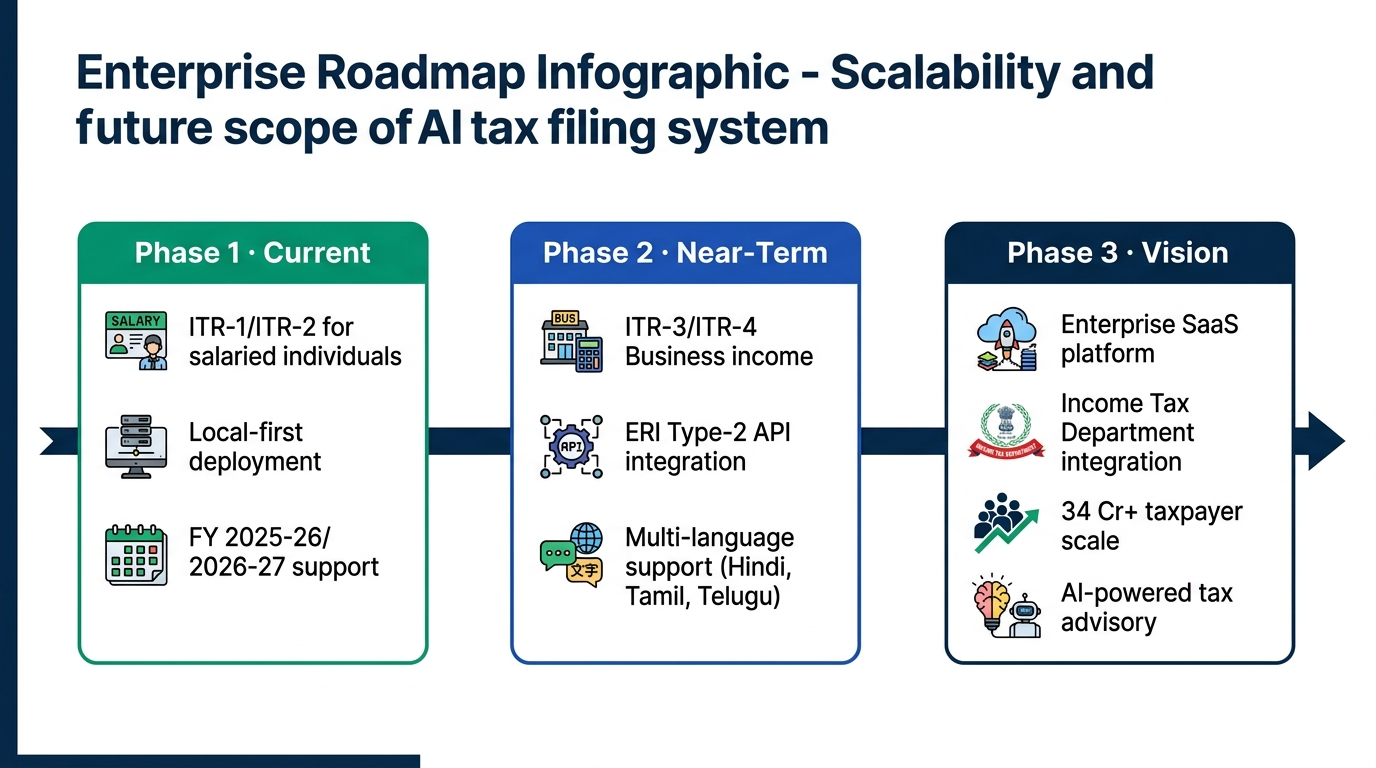
\includegraphics[width=0.95\textwidth]{scalability_future.jpg}
  % ══════════════════════════════════════════════════════════════════════════

  \begin{center}
    \begin{tikzpicture}[
      phase/.style={draw=BorderGray, rounded corners=6pt, fill=white,
                    minimum width=4.2cm, minimum height=4.5cm, inner sep=6pt,
                    text width=3.8cm},
      arrow/.style={-{Stealth[length=4pt]}, ultra thick}
    ]
      % Phase 1
      \node[phase, draw=EmeraldGreen] (p1) at (0,0) {
        {\color{white}\colorbox{EmeraldGreen}{\fontsize{9}{11}\selectfont\bfseries
          ~~Phase 1: Current~~}}\\[4pt]
        {\color{DarkText}\fontsize{8}{10}\selectfont
          {\color{EmeraldGreen}\faIcon{check-circle}}~ITR-1/ITR-2 support\\[2pt]
          {\color{EmeraldGreen}\faIcon{check-circle}}~Salaried individuals\\[2pt]
          {\color{EmeraldGreen}\faIcon{check-circle}}~Local-first deployment\\[2pt]
          {\color{EmeraldGreen}\faIcon{check-circle}}~FY 2025-26 and 2026-27\\[2pt]
          {\color{EmeraldGreen}\faIcon{check-circle}}~8-agent pipeline\\[2pt]
          {\color{EmeraldGreen}\faIcon{check-circle}}~Self-healing loop}
      };

      % Phase 2
      \node[phase, draw=RoyalBlue, right=0.5cm of p1] (p2) {
        {\color{white}\colorbox{RoyalBlue}{\fontsize{9}{11}\selectfont\bfseries
          ~~Phase 2: Near-Term~~}}\\[4pt]
        {\color{DarkText}\fontsize{8}{10}\selectfont
          {\color{RoyalBlue}\faIcon{arrow-circle-right}}~ITR-3/ITR-4 business income\\[2pt]
          {\color{RoyalBlue}\faIcon{arrow-circle-right}}~ERI Type-2 API integration\\[2pt]
          {\color{RoyalBlue}\faIcon{arrow-circle-right}}~Multi-language (Hindi, Tamil)\\[2pt]
          {\color{RoyalBlue}\faIcon{arrow-circle-right}}~PostgreSQL + ChromaDB\\[2pt]
          {\color{RoyalBlue}\faIcon{arrow-circle-right}}~Enhanced OCR pipeline\\[2pt]
          {\color{RoyalBlue}\faIcon{arrow-circle-right}}~Docker deployment}
      };

      % Phase 3
      \node[phase, draw=DeepNavy, right=0.5cm of p2] (p3) {
        {\color{white}\colorbox{DeepNavy}{\fontsize{9}{11}\selectfont\bfseries
          ~~Phase 3: Vision~~}}\\[4pt]
        {\color{DarkText}\fontsize{8}{10}\selectfont
          {\color{DeepNavy}\faIcon{rocket}}~Enterprise SaaS platform\\[2pt]
          {\color{DeepNavy}\faIcon{rocket}}~IT Dept.~API integration\\[2pt]
          {\color{DeepNavy}\faIcon{rocket}}~34 Cr+ taxpayer scale\\[2pt]
          {\color{DeepNavy}\faIcon{rocket}}~AI-powered tax advisory\\[2pt]
          {\color{DeepNavy}\faIcon{rocket}}~GST integration layer\\[2pt]
          {\color{DeepNavy}\faIcon{rocket}}~White-label for ERIs}
      };

      % Arrows
      \draw[arrow, EmeraldGreen] (p1.east) -- (p2.west);
      \draw[arrow, RoyalBlue] (p2.east) -- (p3.west);
    \end{tikzpicture}
  \end{center}
\end{frame}

% ─────────────────────────────────────────────────────────────────────────────
% SLIDE 18: CONCLUSION
% ─────────────────────────────────────────────────────────────────────────────
\begin{frame}
  \slideheader{Conclusion}{India's First Self-Healing Multi-Agent Tax Preparation System}

  \vspace{2mm}
  \begin{columns}[T]
    \begin{column}{0.55\textwidth}
      {\color{DeepNavy}\fontsize{11}{13}\selectfont\bfseries
        What We Built}\\[6pt]

      \featurebullet{project-diagram}{%
        \textbf{8 Specialized AI Agents} orchestrated via LangGraph
        StateGraph with shared immutable state
      }{RoyalBlue}

      \featurebullet{sync-alt}{%
        \textbf{Self-Healing Pipeline} with bounded remediation,
        confidence gating, and targeted error correction
      }{RemediationOrange}

      \featurebullet{balance-scale}{%
        \textbf{Dual-Regime Tax Engines} with deterministic computation,
        breakeven analysis, and CA-grade advisory output
      }{DeepNavy}

      \featurebullet{shield-alt}{%
        \textbf{Complete Auditability} with immutable audit trails,
        per-field evidence, and statutory compliance
      }{EmeraldGreen}

      \featurebullet{file-pdf}{%
        \textbf{Production-Ready Output}: Schema-valid ITR JSON +
        Professional Regime Comparison Advisory PDF
      }{EmeraldGreen}
    \end{column}
    \begin{column}{0.42\textwidth}
      \begin{tikzpicture}
        % Key message box
        \node[draw=RoyalBlue, rounded corners=8pt, fill=LightBlue,
              text width=5.5cm, inner sep=8pt, line width=1.5pt] at (0,0.5) {
          {\color{DeepNavy}\fontsize{11}{13}\selectfont\bfseries
            \faIcon{quote-left}~~Key Message}\\[6pt]
          {\color{DeepNavy}\fontsize{9}{12}\selectfont\itshape
            This system doesn't just compute taxes ---
            it \textbf{extracts}, \textbf{verifies},
            \textbf{self-corrects}, and \textbf{documents}
            the entire process with complete transparency.}\\[6pt]
          {\color{TextGray}\fontsize{8}{10}\selectfont
            Ready for adoption by the Income Tax Department of India
            or integration into large-scale tax technology platforms.}
        };

        % Metrics summary
        \node[draw=EmeraldGreen, rounded corners=6pt, fill=LightEmerald,
              text width=5.5cm, inner sep=6pt] at (0,-3) {
          {\color{DeepNavy}\fontsize{9}{11}\selectfont\bfseries
            Key Metrics Summary}\\[4pt]
          {\color{DarkText}\fontsize{8}{10}\selectfont
            \textbf{98.7\%} extraction accuracy\\
            \textbf{99.9\%} tax calculation accuracy\\
            \textbf{0.96} verification confidence\\
            \textbf{$<$45s} end-to-end processing\\
            \textbf{100\%} audit trail coverage}
        };
      \end{tikzpicture}
    \end{column}
  \end{columns}
\end{frame}

% ─────────────────────────────────────────────────────────────────────────────
% SLIDE 19: THANK YOU
% ─────────────────────────────────────────────────────────────────────────────
\begin{frame}[plain]
  \begin{tikzpicture}[remember picture, overlay]
    % Background
    \fill[white] (current page.south west) rectangle (current page.north east);

    % Top accent
    \fill[DeepNavy] (current page.north west) rectangle
      ([yshift=-3mm]current page.north east);

    % Left stripe
    \fill[RoyalBlue] (current page.north west) rectangle
      ([xshift=4mm]current page.south west);

    % Bottom bar
    \fill[DeepNavy] (current page.south west) rectangle
      ([yshift=14mm]current page.south east);

    % Main content
    \node[anchor=center, text width=12cm] at ([yshift=10mm]current page.center) {
      \centering
      {\color{DeepNavy}\fontsize{36}{40}\selectfont\bfseries Thank You}\\[12pt]
      {\color{RoyalBlue}\rule{4cm}{0.6pt}}\\[12pt]
      {\color{DeepNavy}\fontsize{14}{17}\selectfont\bfseries
        Self-Healing Multi-Agent Tax Preparation System}\\[4pt]
      {\color{TextGray}\fontsize{11}{14}\selectfont
        India's First AI-Powered Autonomous Tax Filing Pipeline}\\[16pt]
      {\color{RoyalBlue}\fontsize{11}{14}\selectfont
        \faIcon{github}~~github.com/PMounindra/self-healing-tax-filing-india}\\[6pt]
      {\color{TextGray}\fontsize{10}{12}\selectfont
        \faIcon{envelope}~~Contact: Team Self-Healing Tax}\\[16pt]
      {\color{RoyalBlue}\rule{6cm}{0.4pt}}\\[8pt]
      {\color{TextGray}\fontsize{9}{11}\selectfont\itshape
        ``LLMs read and classify. Deterministic code decides and computes.''}\\[12pt]
      {\color{TextGray}\fontsize{8}{10}\selectfont
        Built with Python $\mid$ FastAPI $\mid$ LangGraph $\mid$ React $\mid$ Tesseract OCR $\mid$ Ollama}
    };

    % Bottom bar text
    \node[anchor=south, text=white, font=\fontsize{8}{10}\selectfont]
      at ([yshift=3mm]current page.south)
      {Computer-generated advisory. Not tax advice.
       Verify with a qualified chartered accountant before filing.};
  \end{tikzpicture}
\end{frame}

\end{document}
